%%%%%%%%%%%%%%%%%%%%%%%%%%%%% Define Article %%%%%%%%%%%%%%%%%%%%%%%%%%%%%%%%%%
\documentclass[a4paper]{article}
%%%%%%%%%%%%%%%%%%%%%%%%%%%%%%%%%%%%%%%%%%%%%%%%%%%%%%%%%%%%%%%%%%%%%%%%%%%%%%%

%%%%%%%%%%%%%%%%%%%%%%%%%%%%% Using Packages %%%%%%%%%%%%%%%%%%%%%%%%%%%%%%%%%%
\usepackage{geometry}
\usepackage{graphicx}
\usepackage{amssymb}
\usepackage{amsmath}
\usepackage{amsthm}
\usepackage{booktabs}
\usepackage{lipsum}
\usepackage{graphicx}
\usepackage{color}
\usepackage{nth}
\usepackage{bm}
\usepackage{caption}
\usepackage{subcaption}
\usepackage{url}
\usepackage{array}
\usepackage{multirow}
%%%%%%%%%%%%%%%%%%%%%%%%%% Page Setting %%%%%%%%%%%%%%%%%%%%%%%%%%%%%%%%%%%%%%%
\geometry{a4paper}

%%%%%%%%%%%%%%%%%%%%%%%%%% Define some useful colors %%%%%%%%%%%%%%%%%%%%%%%%%%
\definecolor{ocre}{RGB}{243,102,25}
\definecolor{mygray}{RGB}{243,243,244}
\definecolor{deepGreen}{RGB}{26,111,0}
\definecolor{shallowGreen}{RGB}{235,255,255}
\definecolor{deepBlue}{RGB}{61,124,222}
\definecolor{shallowBlue}{RGB}{235,249,255}
%%%%%%%%%%%%%%%%%%%%%%%%%%%%%%%%%%%%%%%%%%%%%%%%%%%%%%%%%%%%%%%%%%%%%%%%%%%%%%%

%%%%%%%%%%%%%%%%%%%%%%%%%% Macros %%%%%%%%%%%%%%%%%%%%%%%%%%%%%%%%%%%%%%%%%%%%%
\DeclareMathOperator{\Lagr}{\mathcal{L}}
%%%%%%%%%%%%%%%%%%%%%%%%%%%%%%%%%%%%%%%%%%%%%%%%%%%%%%%%%%%%%%%%%%%%%%%%%%%%%%%


\begin{document}
  % custom title page
  \begin{titlepage}
  \begin{center}

    \vspace*{1cm}

    \textbf{\LARGE
    % Training and Deploying Computer Vision Models for Indoor Localisation
    % Exploring Deep Learning for Indoor Localisation: A Study on Room-Level Accuracy
    Navigating Indoors with Computer Vision: Exploring Deep Learning Approaches
    for Room-Level Indoor Localisation
    % Deep Learning for Accurate Room-Level Indoor Localisation: Feasibility and Evaluation
    % Enhancing Indoor Spatial Awareness: Deep Learning Approaches for Room-Level
    % Indoor Localisation
    }

    \vspace{1.5cm}

    % author
    \begin{minipage}[t]{5cm}
      \centering
      \textbf{Mika Senghaas} (Author) \\
      IT University of Copenhagen \\
      \textit{jsen@itu.dk}
    \end{minipage}
    \hspace{1cm}
    \begin{minipage}[t]{5cm}
      \centering
      \textbf{Stella Grasshof} (Supervisor) \\
      IT University of Copenhagen \\
      \textit{stgr@itu.dk}
    \end{minipage}

    \vfill

    % degree
    A Thesis presented for the Degree of \\
    \textbf{Bachelor of Science in Data Science}

    \vspace{0.8cm}

    
\includegraphics[width=0.4\textwidth]{figures/itu.jpg}

    \vspace{0.8cm}

    \textbf{IT University of Copenhagen}\\
    Computer Science Department\\
    \vspace{.5cm}
    May, 15th 2023

  \end{center}
\end{titlepage}

  \newpage

  % table of contents, list of tables, list of figures
  \tableofcontents
  \listoftables
  \listoffigures
  \newpage

  \begin{abstract} % (fold)
    \lipsum[1]
  \end{abstract}

  \section{Introduction}
  \label{sec:introduction}

  Knowing where you are is crucial for human life. For as long as humans have
  lived, they have tried to determine their position on the earth. First, by
  observing the position of the sun, and later by using the stars. With advances
  in technology in the second half of the \nth{20} century, specifically the
  invention and commercialisation of GPS (Global Positioning System), a
  satellite-based localisation system, localisation has become more efficient
  and accurate than ever before. Gradual commercialisation led to the technology
  rapidly transforming entire industries and personal navigation systems. Today,
  outdoor localisation is widely considered a \textit{solved problem}.

  The same cannot be said for indoor localisation. Because the transmitted radio
  signals sent out by the satellites in the GPS systems are not strong enough to
  penetrate through walls and struggle with reflections from large buildings,
  the technology yields inaccurate results at best, and often becomes
  dysfunctional in indoor spaces.

  Finding alternative solutions to provide an accurate, cheap and robust indoor
  localisation systems has been a main focus of research in the past decades,
  and is becoming increasingly important in the light of the ongoing urbanisation
  of our living spaces and the emergence of autonomous robots and vehicles in
  our everyday life. Nonetheless, commercial applications are still rare and not
  unified in their approach.

  Decades of research have led to the development of a variety of different
  indoor localisation technologies. Hardware-based systems use radio signals,
  transmitted by beacons, like Bluetooth, and Ultra-Wideband
  (UWB) or Wi-Fi, to localise an agent in a known environment. Software-based
  systems, like Simultaneous Localisation and Mapping (SLAM) algorithms, use
  sensors, like cameras or distance-measuring laser sensors, to localise an
  agent, while simultaneously creating a map of the environment. 

  However, hardware-based system require an expensive initial setup, continuous
  maintenance of the beacons, and are often not feasible in large environments,
  like shopping malls, or in environments that are frequently changing, like
  offices. SLAM algorithms, on the other hand, require a meticulously
  handcrafted pipeline of feature detection, feature matching, and pose
  estimation that has to be fine-tuned for each indoor space, to achieve
  outstanding results. Furthermore, some SLAM algorithms require specific types
  of sensors to be used, which are not available to use in all environments.

  % run on: make it run on commercial mobile devices (computational limitation
  % and limited to a single camera)
  % requiring minimal initial setup in the environment and the devices
  % TODO: mention that the project works under the assumption that for some
  % applications it is sufficient to know the position of the agent with a
  % meter, instead of centimeter accuracy. In these cases, a versatile and
  % simple solution is preferable 
  % TODO: give an example of such an application with mobile indoor navigation
  % applications

  In an attempt to overcome the limitations of the aforementioned indoor
  localisation technologies, and to provide a simple, unified indoor
  localisation system this thesis proposes a novel approach to indoor
  localisation, by framing the problem of indoor localisation as a simple
  classification task. In our setup, location labels are continuously predicted
  from a stream of images, using different types of modern deep neural networks,
  such as convolutional neural networks (CNNs) and recurrent neural networks
  (RNNs). With the advances in the computational power of modern mobile devices,
  the pipeline is proven to provide real-time estimates of the agent's position
  in the environment. Furthermore, the proposed method requires minimal initial
  setup in the environment and the devices, and is therefore suitable for
  commercial applications.

  In this thesis we describe the data collection, model architecture, training
  procedure, and then rigorously evaluate the proposed method in three
  dimensions.

  \begin{itemize}
    \item \textbf{Accuracy:} Are the location estimates correct? 
    \item \textbf{Robustness} Are the location estimates correct when
      encountering noise?
    \item \textbf{Efficiency:} How much data needs to be collected to train
      high-performance models? How quick is the inference times?
  \end{itemize} 

  % section introduction (end)

  \section{Background} % (fold)
  \label{sec:background}

  % Localisation is crucial for human life. We need to know where we are and we
  % need technology to help us determine this, in the case when we cannot.

  % importance of localisation
  Producing accurate, robust and cheap localisation systems is not a novel task,
  but has been a focus of research at the intersection of robotics, computer
  vision and machine learning for decades.

  % SLAM
  Amongst the most promising approaches are SLAM (Simultaneous Localisation and
  Mapping) algorithms. SLAM algorithms aim to localise an agent inside an
  unknown environment, while simultaneously building a consistent map of the
  environment. There exist a variety of different approaches to SLAM, depending
  on the type of sensors that are used for estimating position and mapping the
  environment. For example, Visual SLAM (V-SLAM) algorithms use camera input,
  and LidarSLAM algorithms use distance-measuring laser sensors.
  Initial proposal of such algorithms use a pipeline of feature detection, 
  feature matching, and pose estimation to estimate the position of the agent
  and the environment. 

  The methodology most related to our approach are monocular V-SLAM algorithms,
  which use a single camera to estimate the position of the agent. The very
  first monocular feature-based V-SLAM algorithms is called
  MonoSLAM~\cite{mono-slam} and was proposed in 2007. The researchers proved
  that their approach is capable of simultaneously localising an agent and
  mapping an environment, using a single camera. Thus, overcoming the main
  challenge of inaccurate depth estimation using a single camera.

  Since then, many adjustments and optimisation have been proposed to the
  algorithm to make it more robust and accurate. For example, the
  ORB-SLAM~\cite{orb-slam} algorithm uses a bag-of-words approach to feature
  matching, and the PTAM~\cite{ptam} algorithm uses a parallel tracking and
  mapping approach to improve the accuracy of the algorithm. 

  With machine and deep learning becoming more and more popular in the past
  decade, many researchers have started to apply these techniques to SLAM
  algorithms. For example, the DeepVO~\cite{deep-vo} algorithm uses a
  convolutional neural network to estimate the camera pose from a sequence of
  images. All the above mentioned approaches are similar to our approach in that
  they use deep learning at some part of the pipeline, but differ in that simply
  replace the original components in a SLAM pipeline, such as feature
  extraction, feature matching, or pose estimation, with a deep neural network,
  whereas we use deep learning to learn a mapping from images to location
  

  % TODO: section about some of the inherent challenges of image classification
  % of location based of frames of indoor spaces
  % lighting, camera angle, temporal
  %objects, humans crossing the camera's view, labels.

  % TODO: mention the success of deep learning in computer vision (resnet, ...)

  % section background (end)

  \section{Methodology} % (fold)
  \label{sec:methodology}

  The project is an end-to-end machine learning pipeline, meaning that it
  starts with the collection of data, and ends with the deployment of a
  production-ready model. 

  \subsection{Data Collection} % (fold)
  \label{sub:data-collection}

  % how does that data need to look?
  % where was the data collected (why not online data set)
  % when was the data collected
  % how the data was collected
  % how was the data annotated

  Framing the problem of indoor localisation as a classification task requires a
  labelled data set, which consists of sequentially-arranged pairs of video
  frames and location labels. A single video clip $C$ consists of a sequence of
  $n$ frames $x_0, ..., x_n$ and a sequence of $n$ location labels $y_0, ...,
  y_n$, where the $i$-th pair of the sequence is the tuple $(x_i,y_i)$ and
  denotes the location at a specific frame. A single frame $x_i$ is a RGB image,
  represented as a three-dimensional tensor of shape $3 \times H \times W$,
  where $H$ and $W$ are the height and width of the image, respectively. A
  single location label $y_i$ is a scalar value, which identifies the location
  of the agent at the time of the frame. 

  % place of data collection
  The data set was collected from a single camera of a mobile
  device~\footnote{iPhone 11 Pro recording at 30 FPS with 2426x1125 HD
  resolution} that was hand-held by a human agent while walking around an indoor
  building. The chosen location for the data collection was the main building of
  the Southern Campus of the Copenhagen University (Danish: K\o{}benhavns
  Universitet, KU) in Copenhagen S, Denmark. The building is a large
  multi-storey building with a total of six floors, and is used for teaching and
  research purposes. The location was deemed ideal for this initial research, as
  it both has distinctive indoor features (e.g. coloured walls, unique
  structures, etc.), but also poses a challenge for the model, for example, due
  to the similarity of the floor plan across floors.
  For the scope of this project, the data collection was limited to the first
  two floors. The publicly accessible areas were separated into 21 different
  location labels (Figure~\ref{fig:map}), in close correspondence to the
  official building's floor plan. The location labels were denoted with
  descriptive identifiers (e.g. \texttt{Ground Floor Atrium},
  \texttt{First Floor Red Area}, etc.)

  % figure
  \begin{figure}[ht]
    \centering
    % subfigure
    \begin{subfigure}[b]{0.49\linewidth}
      \centering
      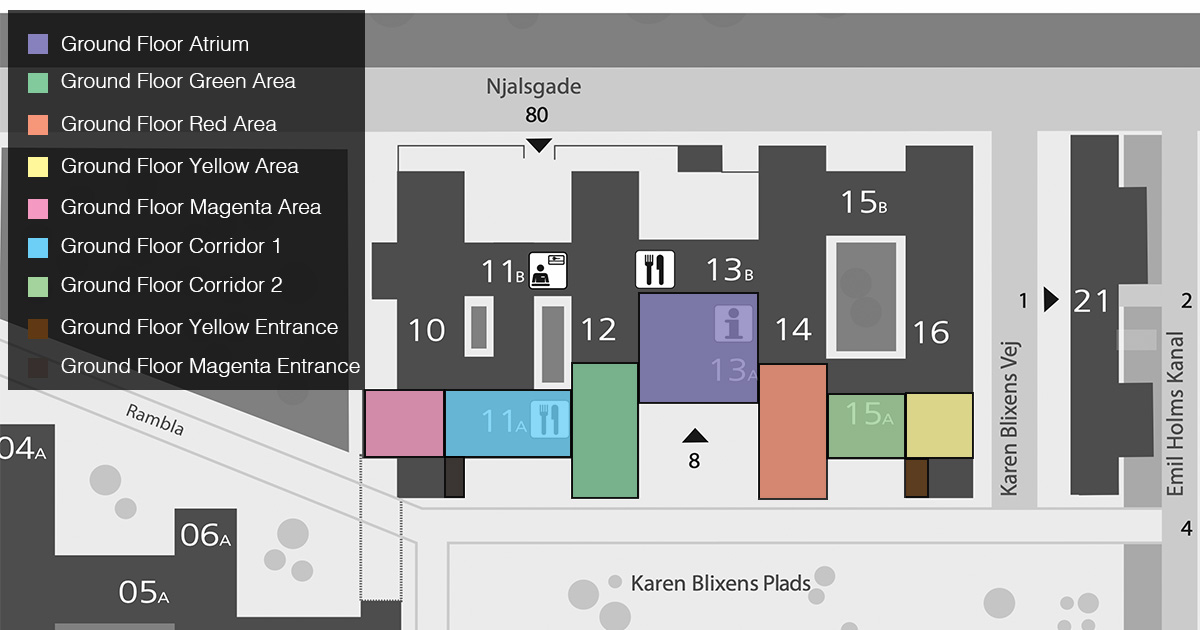
\includegraphics[width=\linewidth]{figures/map-ground-floor.jpg}
      \caption{Ground Floor}
      \label{fig:map-ground-floor}
    \end{subfigure}
    \hfill
    % subfigure
    \begin{subfigure}[b]{0.49\linewidth}
      \centering
      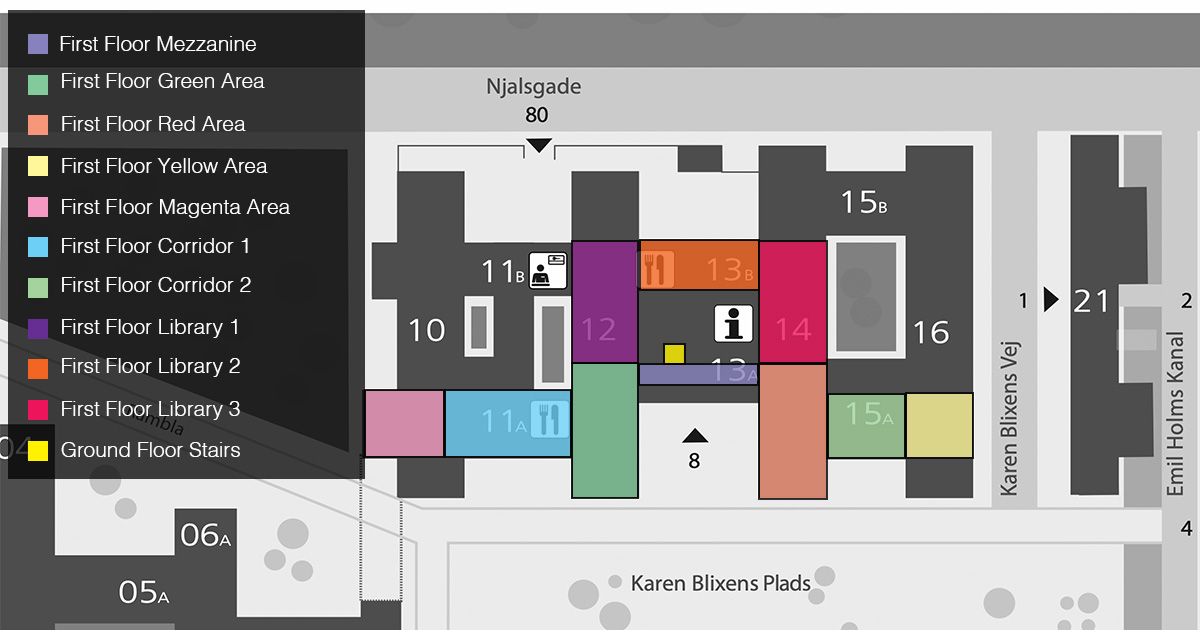
\includegraphics[width=\linewidth]{figures/map-first-floor.jpg}
      \caption{First Floor}
      \label{fig:map-first-floor}
    \end{subfigure}
    \caption{Map of KU Southern Campus Main Building with Location Labels}
    \label{fig:map}
  \end{figure}

  To match the location labels to the video footage, each clip $C$ was manually
  annotated by denoting the starting and ending time stamps of a location label.
  The information was stored in a standardised format and later used in the
  pre-processing of clips into frame-location pairs.

  % statistics of the data
  A total of 53 video clips were recorded, with an average duration of ~57s,
  amounting to a total number of $\sim$ 50 minutes of footage. Out of the total
  53 video clips that were recorded, 37 were used for training and 16 were used
  for validation. Table~\ref{tab:data-stats} shows more statistics of the raw
  data in the two different splits.

  \begin{table}[ht]
    \centering
    \begin{tabular}{llll}
    \toprule
    \bfseries Split & Total Clips & Total Seconds & Total Minutes \\
    \midrule
    Training & 37 &  2240 & 37 \\
    Testing & 16 & 783 & 13 \\
    \bottomrule
    \end{tabular}
    \caption{Statistics of the Raw Data in Training and Testing Splits}
    \label{tab:data-stats}
  \end{table}

  % time of data collection
  An ideal model learns robust indoor features that are invariant to natural 
  variations in the indoor space from training data collected in a minimal time
  span, as this minimises the initial cost and effort for data collection.
  To evaluate the model's robustness towards these variations, a different
  philosophy was adopted for the collection of training and testing data.

  While the 37 training clips were recorded on just two days, the 16 testing
  clips were recorded on four different days, two to four weeks after the
  initial training data collection. This was done to make the testing data
  closer resemble real-world scenarios, and thereby make the testing metrics
  more robust.
  
  % TODO: figure about the time of data collection (side-by-side, one where hue
  %       denotes the split and the other where hue denotes the clips per day)

  % subsection data-collection (end)

  \subsection{Data Preprocessing} % (fold)
  \label{sub:data-preprocessing}

  The raw video clips and manual annotation of location labels, had to be
  pre-processed before they could be used for training deep learning models.

  The video footage was resized to a resolution of 224x224 pixels, which is the
  input resolution of most modern foundation models for image and video
  classification, which were used in this project. Furthermore, it decreases the 
  total data amount significantly, which allowed for less disk usage and faster
  loads into memory during training.

  Next, instead of extracting all 30 frames per second, the video footage was
  downsampled to a much lower frame rate of 1 FPS. This was done to reduce the
  total data amount, and to reduce over-fitting of the model to the training
  data. It was hypothesised, that because of the strong local dependency of
  consecutive frames, consecutive frames are highly correlated, thus including
  such frames does not introduce any additional variance, but redundancies that
  are harmful for the model's generalisation ability. Empirical experiments
  confirmed that downsampling indeed reduces over-fitting, and was therefore
  adopted across all experiments.

  Finally, the pre-processed video footage was aligned with the manual location
  labels by extracting a frame per second from the video and matching it against
  the location label that was active at that time. After pre-preprocessing,
  there exist pairs $(x_i, y_i)$, where $x_i$ is pre-processed, extracted frame
  of size 224x224 pixels, and $y_i$ is the corresponding location identifier.
  The frames were stored in a way that allowed for easily sampling both a random
  frame-location pair $(x_i, y_i)$ for image classification models, or a
  sequence of consecutive $n$ frames from a clip $([x_0, \ldots, x_n], [y_i,
  \ldots y_n])$ for video classification models. Here the sequence of frames was
  represented as a 4D-tensor of size $n \times 3 \times 224 \times 224$.

  Figure~\ref{fig:preprocessed-data} shows $n=4$ consecutive frame-location
  label pairs after preprocessing. As can be seen, even at a frame rate of 1
  FPS, neighbouring frames are still similar to each other. Further, the
  annotation at the transition from one location to another was often difficult
  to determine, as one could annotate strictly according to the device position
  or the view of the camera. This likely resulted in some frames being annotated
  with the wrong location label.

  % figure
  \begin{figure}[ht]
    \centering
    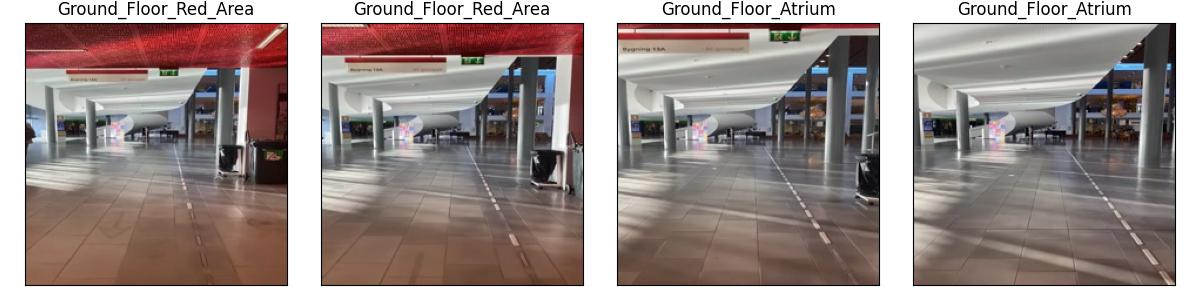
\includegraphics[width=\linewidth]{figures/data-example-batch.jpg}
    \caption{Examples of preprocessed frame-location pairs}
    \label{fig:preprocessed-data}
  \end{figure}

  % TODO: frame preprocessing: tofloat(), normalisation, standardisation
  
  % subsection data-preprocessing (end)

  \subsection{Models} % (fold)
  \label{sub:models}

  A deep learning model is supposed to learn a function $f: X \rightarrow Y$,
  where $X$ represents the input space and $Y$ the output space. By having
  framed the task of indoor localisation as a classification problem, the output
  space is the discrete set of location labels, $Y = \{l_1, \ldots, l_n\}$.
  Two approaches are viable for the input space $X$:

  \begin{enumerate}

    \item \textbf{Image Classification}: The input space $X$ is a single frame,
      $(3, H, W)$ and the output space is a single location label $y \in Y$.
      The model treats consecutive frames independently, and
      therefore disregards the temporal dimension of the video.

    \item \textbf{Video Classification}: The input space $X$ is a sequence of
      $N$ frames, $(x_1, \ldots, x_n)$, and the output space $Y$ is a sequence
      of $N$ location labels, $(y_0, \ldots, y_n)$, where each $y_i \in Y$. The
      model considers the temporal dimension of the video, and learns to
      classify the location label of a sequence of frames. In reality, the input
      sequence has a maximum context length $K$, meaning that the model
      continuously predicts on the previous $K$ frames.

  \end{enumerate}

  % explain that what CNN architecture is 
  % explain that what RNN architecture is
  % dominate computer vision tasks and are therefore used here
  % introduce notion of cnn module (any module that takes a single frame and
  % outputs a high-level feature representation) and rnn module (any module that
  % is capable of taking a sequence of frames and outputs a high-level feature
  % representation for each of them)

  % explain why video classifiers and transformers are disregarded

  \begin{figure}[ht]
    \centering
    \begin{subfigure}[b]{0.42\linewidth}
      \centering
      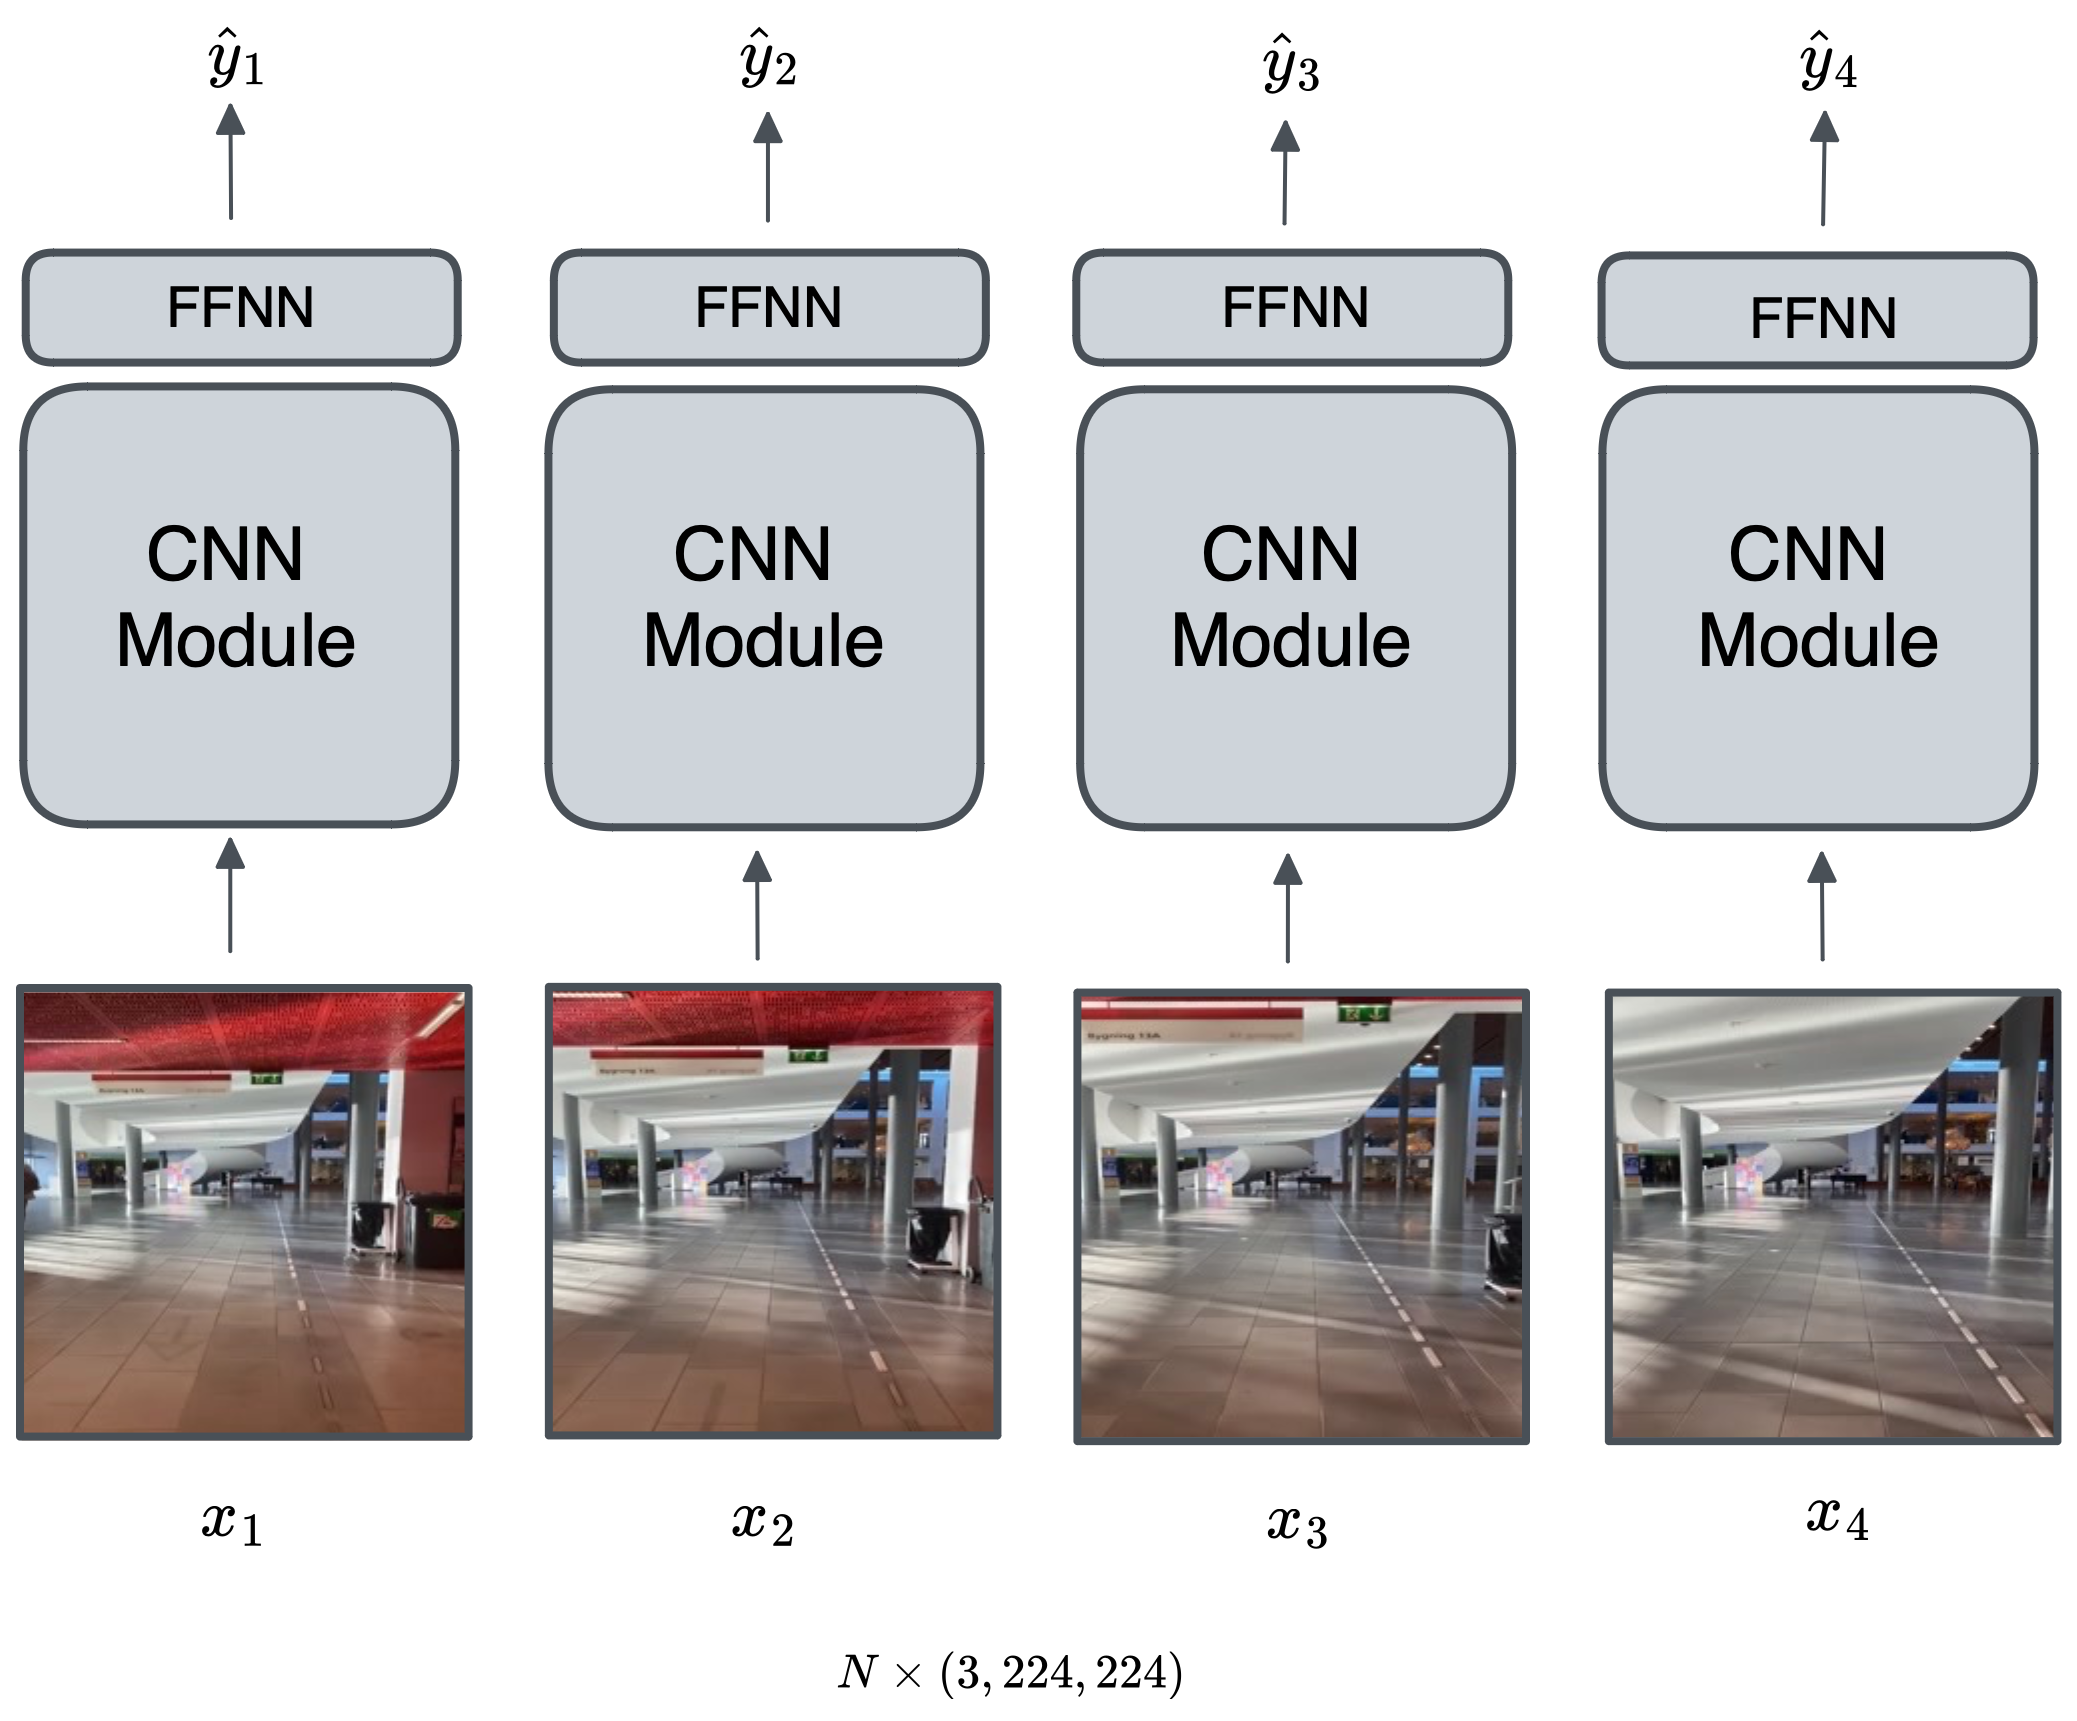
\includegraphics[width=\linewidth]{figures/cnn-architecture.png}
      \caption{Image Classification Architecture}
      \label{fig:cnn-architecture}
    \end{subfigure}
    \hfill
    \begin{subfigure}[b]{0.42\linewidth}
      \centering
      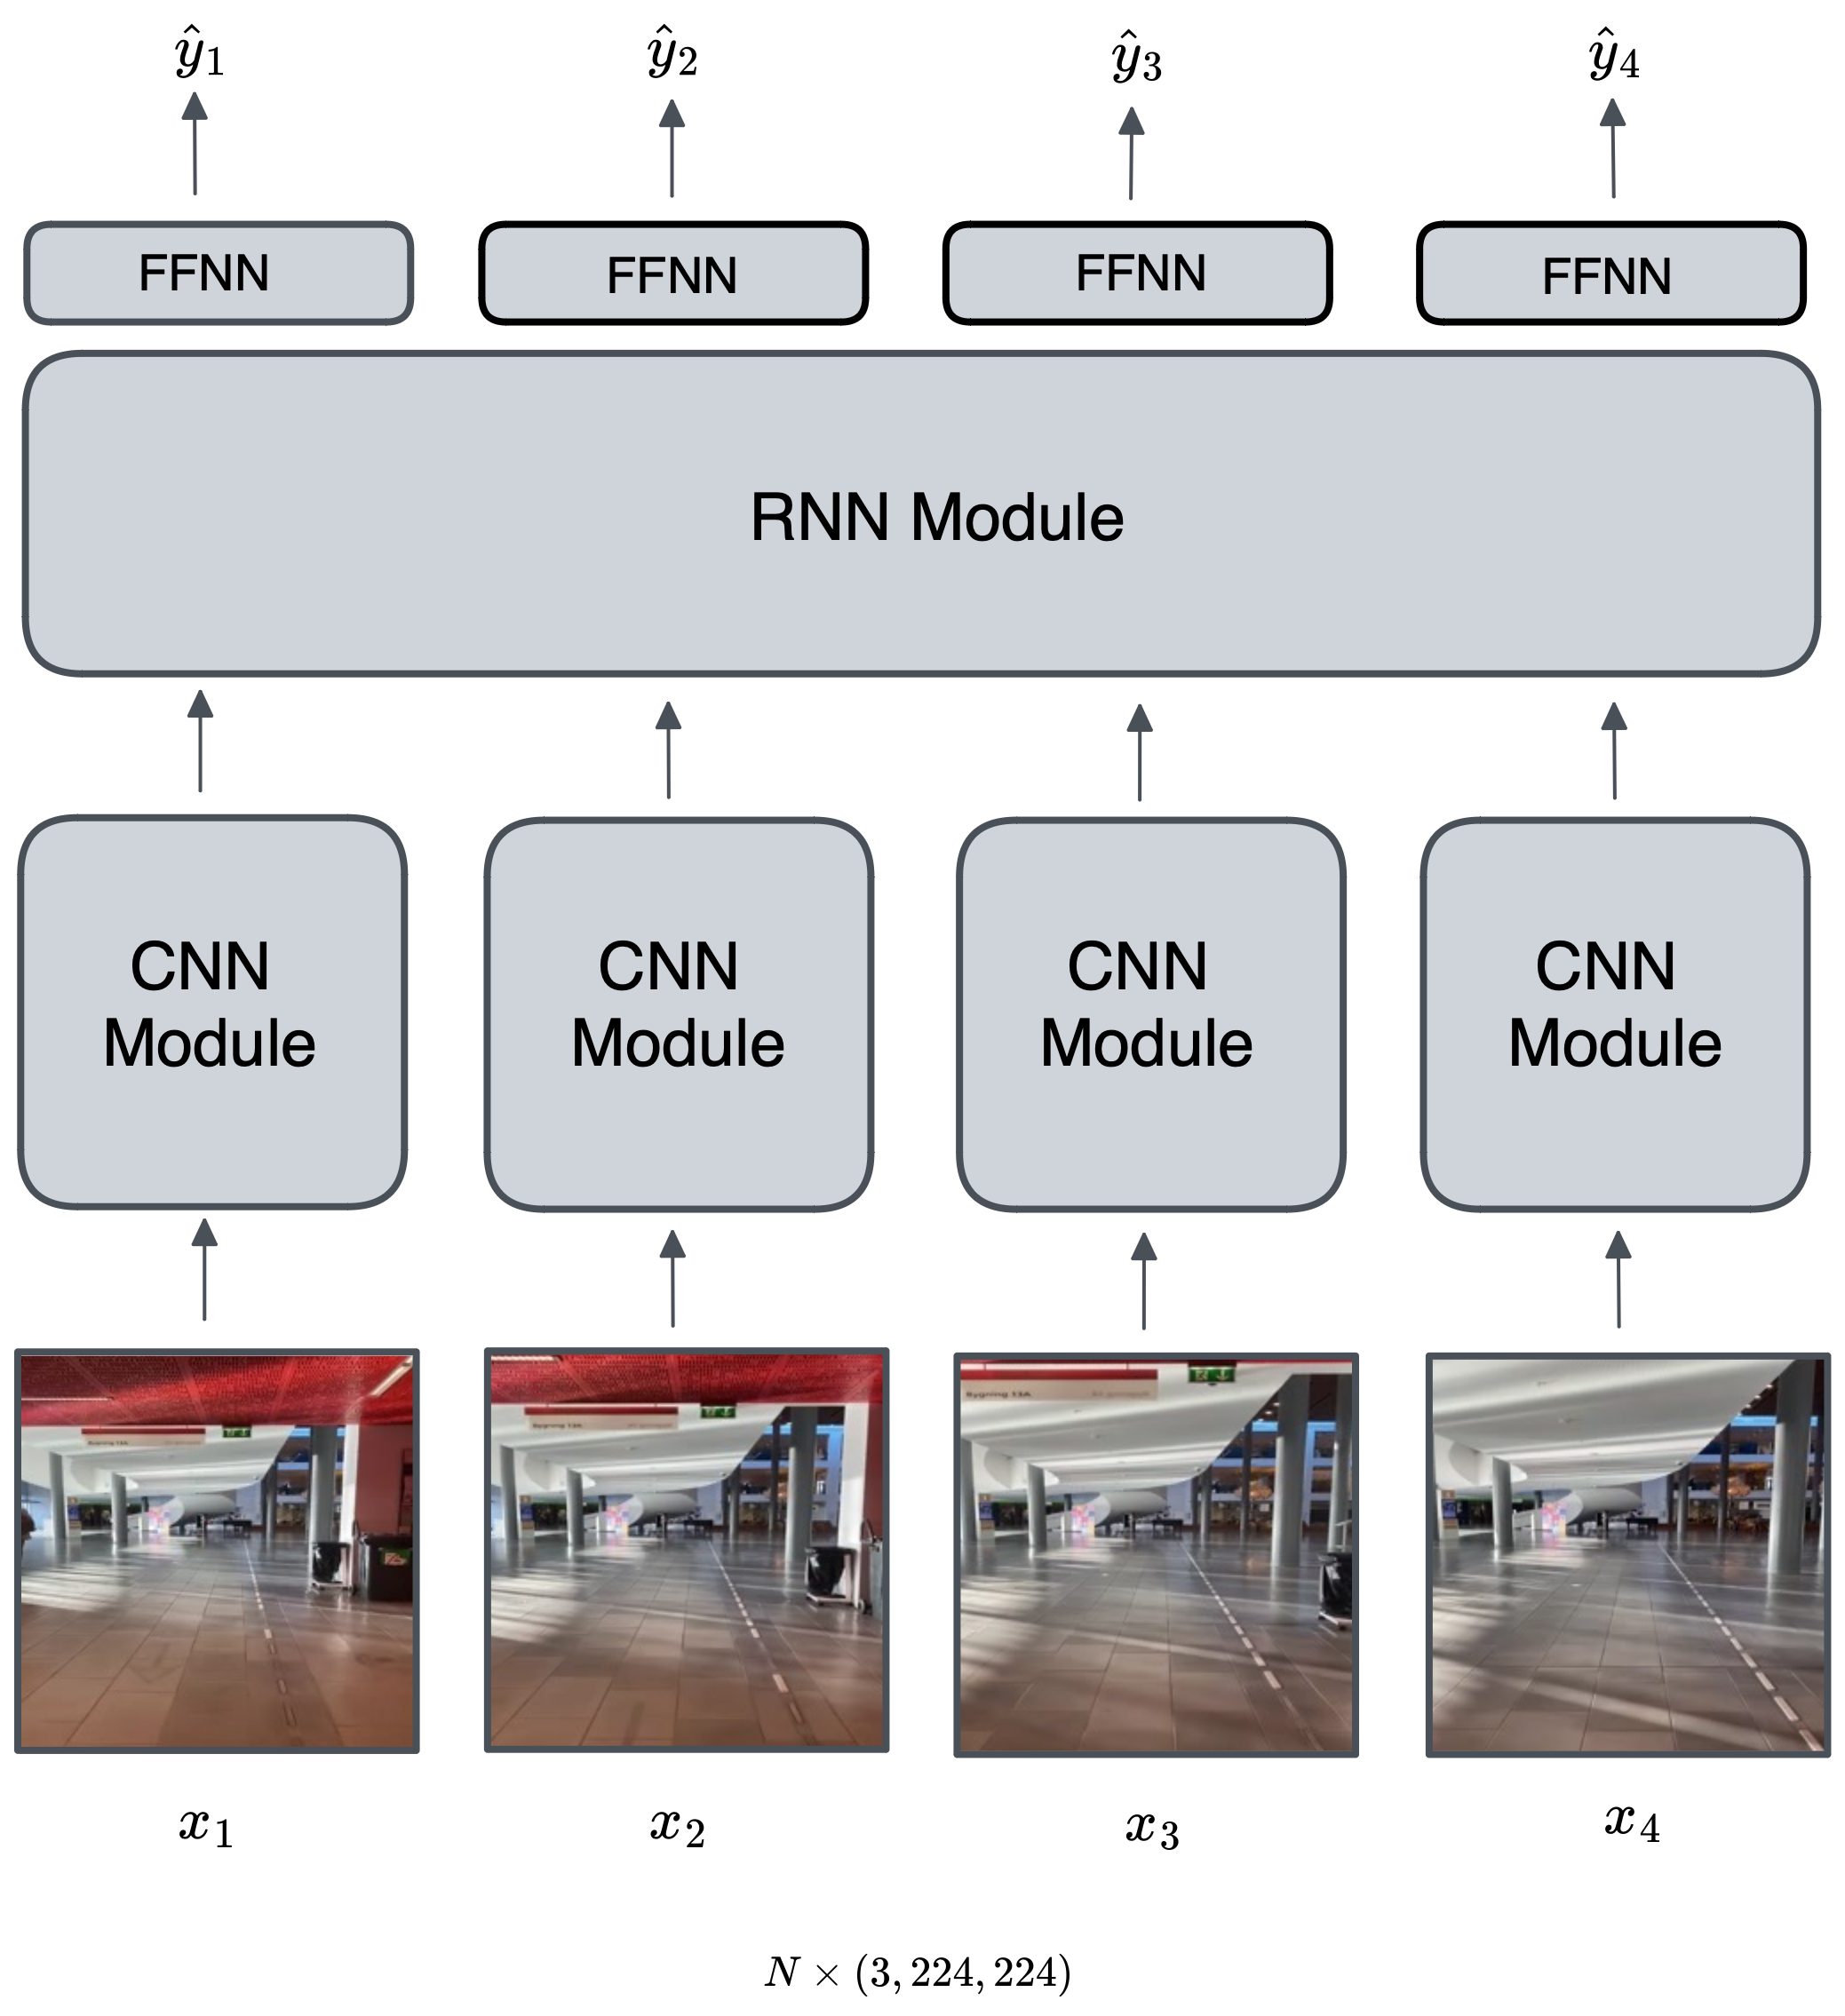
\includegraphics[width=\linewidth]{figures/rnn-architecture.png}
      \caption{Video Classification Architecture}
      \label{fig:rnn-architecture}
    \end{subfigure}
    \caption{Model Architectures}
    \label{fig:model-architectures}
  \end{figure}

  Figure~\ref{fig:model-architectures} shows the high-level architecture of the two
  approaches. For an image classification model, a sequence of $N$ (here $N=4$)
  frames are independently fed into a convolutional neural network (CNN), which
  outputs a feature vector for each frame. CNNs are a class of deep neural
  networks that are applied to analyse visual imagery. They are composed of
  several layers of alternating convolutional and pooling filters, which are
  applied to the input image to extract high-level feature representations.
  These high-level feature representations are then fed into a fully connected
  neural network (FCNN), which outputs a probability distribution over the
  location labels.

  For a video classification model, all $N$ consecutive frames are independently
  passed through a CNN module. The sequence of high-level feature
  representations is then fed into a recurrent neural network (RNN), which
  outputs a probability distribution over the location labels for each frame by
  placing a fully connected layer (classification head) to the output vector
  associated to each frame in the RNN module. A recurrent neural network (RNN)
  is a class of deep neural networks that is applied to analyse sequential data.
  Although they are mostly applied to natural language processing tasks, the
  generality of their architecture allows to also apply them to computer vision
  tasks with sequential data, such as a sequence of frames in video
  classification. For each input $x_i$ in a sequence of inputs, the RNN computes
  an output as a function of the current input $x_i$ and a hidden state
  $h_{i-1}$ that is computed as a function of all previous inputs. In that way,
  the RNN can learn to model the temporal dependencies between frames, e.g.
  consider that all previous frames were predicted to be at one specific
  location, and therefore the current frame is also likely to be at that
  location.

  To evaluate the performance of both approaches, a selection of well-performing
  CNN and RNN modules were chosen, and combined to form different image and
  video classifiers. The modules, alongside meta information about their number
  of parameters, size in Megabyte (MB) and GFLOPS (Giga Floating Point
  Operations per Second) are provided in Table~\ref{tab:modules}. Generally
  speaking, smaller model sizes are preferred, as they are faster to train and
  during inference and require less memory, making them more suitable to be
  deployed on low-resource devices like mobile phones and embedded devices. It
  is expected that more complex, larger models will perform better, so the goal
  is to choose the smallest model that works well enough to perform the task
  with sufficient accuracy.

  \begin{table}[ht]
    \centering
    \begin{tabular}{rllll}
      \toprule
      Type & Name & \#Params & GFLOPS & Size (MB) \\
      \midrule
      \textbf{CNN Module} & Resnet18~\cite{resnet} & 11.6M & 1.81 & 44.7 \\
                          & Resnet50~\cite{resnet} & 25.6M & 4.09 & 99.8 \\
                          & MobileNet-V3 & 2.5M & 0.06 & 9.8 \\
                          & Alexnet & 61.1M & 0.71 & 233.1 \\
      \midrule
      \textbf{RNN Module} & RNN & 0.26 & N/A & 1.04 \\
                          & LSTM & 1.05 & N/A & 4.2 \\
      \bottomrule
    \end{tabular}
    \caption{CNN and RNN Modules}
    \label{tab:modules}
  \end{table}

  By replacing the final fully connected layer of the CNN with a linear layer
  with $N$ outputs, where $N$ is the number of location labels, each CNN module
  can be used as an image classifier. Because the different RNN modules expect a
  one-dimensional input for each element in the input sequence of frames, the
  RNN modules are combined with a CNN module to form a CNN-RNN architecture.
  Given the 4 different CNN modules and the 2 different RNN modules, 8 different
  CNN-RNN architectures were formed for the video classification approach. The
  list of all image and video classifiers that were evaluated is provided in
  Table~\ref{tab:models}.


  \begin{table}[ht]
    \centering
    \begin{tabular}{lll}
      \toprule
      \bfseries Name & \bfseries CNN Module & \bfseries RNN Module \\
      \midrule
      resnet18 & ResNet18 & - \\
      resnet50 & ResNet50 & - \\
      mobilenet\_v3\_small & MobileNet-V3 & - \\
      alexnet & AlexNet & - \\
      \midrule
      resnet18-rnn & Resnet18 & RNN \\
      resnet50-rnn & ResNet50 & RNN \\
      mobilenet\_v3\_small-rnn & MobileNet-V3 & RNN \\
      alexnet-rnn & AlexNet & RNN \\
      resnet18-lstm & Resnet18 & LSTM \\
      resnet50-lstm & ResNet50 & LSTM \\
      mobilenet\_v3\_small-lstm & MobileNet-V3 & LSTM \\
      alexnet-lstm & AlexNet & LSTM \\
      \bottomrule
    \end{tabular}
    \caption{List of all Models}
    \label{tab:models}
  \end{table}

  % subsection models (end)

  \subsection{Training} % (fold)
  \label{sub:training}

  All models were implemented using the PyTorch framework~\cite{pytorch} and the
  training was performed locally on a MacBook Pro M1 with 16GB of memory and
  MPS-acceleration enabled (where possible\footnote{MobileNet-V3-based models do
  not support GPU acceleration}) to allow for fast experiment iteration. The
  loss function $\mathcal{L}$ used for all models was cross-entropy loss
  (Equation~\ref{eq:cross-entropy}), which
  is a standard loss function for multi-class classification problems.

  \begin{equation}
    \mathcal{L}(\hat{y},y) = -\sum_{i=1}^{K} y_i \log(\hat{y}_i)
    \label{eq:cross-entropy}
  \end{equation}

  % TODO: compare to pytorch cross-entropy loss (is it the same? what is the
  % difference to nll?)
  Here, $\hat{y}$ is the predicted probability distribution over the $K$ classes
  and $y$ is the one-hot encoded ground truth label. The models were trained
  using the AdamW~\cite{adamw} optimiser with default parameters, except for the
  learning rate, which was set to a constant of $1e^{-4}$. Step-wise learning
  rate scheduling was used for all models, which reduced the learning rate by a
  factor of 10 every 5 epochs. The batch size was set to 32 for all image
  classifiers and 8 for all video classifiers for memory-optimal training.
  Unless otherwise specified, all image and video classifiers were trained with
  the same set of training hyper-parameters, which are specified in Table
  \ref{tab:default-hyperparams}. 

  \begin{table}[ht]
    \centering
    \begin{tabular}{rllll}
      \toprule
      Classifier & Batch Size & Epochs & Optimiser & Learning Rate Scheduler \\
      \midrule
      \bfseries Image & 32 & 10 & AdamW ($\gamma=1e^{-4}$) & Step-LR
      ($\gamma=1e^{-1}, s=5$) \\
      \bfseries Video & 8 & 10 & AdamW ($\gamma=1e^{-4}$) & Step-LR
      ($\gamma=1e^{-1}, s=5$) \\
      \bottomrule
    \end{tabular}
    \caption{Default Hyperparameters for Image and Video Classifiers}
    \label{tab:default-hyperparams}
  \end{table}

  %   (end)

  \subsection{Evaluation} % (fold)
  \label{sub:evaluation}

  The goal of the evaluation is to have a rigorous comparison of the different
  models and to determine the best model for the task of location
  classification. In this context, a ``well-performing'' model is not just the
  model that is most accurate in most cases, but also the model that is most
  robust to a wide-range of different natural variations that can occur and that
  is efficient. To achieve this, a series of \textit{quantitative} and
  \textit{qualitative} experiments are performed on the models, which are then
  used in Section~\ref{sec:results} and Section~\ref{sec:discussion}.

  \textbf{Quantitative Experiments.} To quantitatively assess the performance of
  the model on the task of location classification, the models were evaluated on
  the test set using a wide-range of different performance metrics. To assess
  the overall accuracy of the model, two metrics are computed:
  \textbf{Multi-class Accuracy} (Equation~\ref{eq:accuracy}) is the most
  wide-spread performance metric in classification task and is defined as the
  number of correct predictions divided by the total number of predictions.
  It gives a good first indication for the overall performance of the model, but
  can be misleading in cases where the dataset is imbalanced.

  \begin{equation}
    \text{Multi-class Accuracy} = \frac{1}{N} \sum_{i=1}^{N} \mathbb{I}(y_i =
    \hat{y}_i) 
    \label{eq:accuracy}
  \end{equation}

  Here, $\mathbb{I}$ is an indicator that is 1 if the condition is true and 0
  otherwise. On top of the standard, multi-class accuracy, a variant of the
  formula, the \textbf{Top-3 Multi-class Accuracy} is also computed, which
  counts a prediction as correct if the correct label is one of the top-3
  predicted labels.

  As some location labels are underrepresented in the dataset due to the natural
  variation in size of the different locations, the \textbf{Macro F1-Score} is
  used to compute a more fine-grained metric. The Macro F1-Score is the average
  of the class-specific F1-scores, which are defined as the harmonic mean of
  precision $P_i$ and recall $R_i$ (Equation~\ref{eq:macro-f1}).

  \begin{equation}
    \text{Macro F1-Score} = \frac{1}{N} \sum_{i=1}^{N} \frac{2 \cdot P_i \cdot 
    R_i}{P_i + R_i}
    \label{eq:macro-f1}
  \end{equation}

  Here, $P_i$ and $R_i$ are the precision and recall for class $i$, which are 
  defined as follows (Equation~\ref{eq:precision}) and (Equation~\ref{eq:recall}).

  \begin{equation}
    P_i = \frac{TP_i}{TP_i + FP_i}
    \label{eq:precision}
  \end{equation}

  \begin{equation}
    R_i = \frac{TP_i}{TP_i + FN_i}
    \label{eq:recall}
  \end{equation}

  Here, $TP_i$ is the number of true positives for class $i$, $FP_i$ is the
  number of false positives for class $i$ and $FN_i$ is the number of false
  negatives for class $i$. 

  On top of the standard metrics for classification, efficiency of the model is
  crucial for usability of the system on low-resource devices, such as mobile
  phones. For this reason, the \textbf{Inference Time} per sample is measured, 
  the \textbf{GFLOPS} per predicted sample is computed and the \textbf{Model
  Size} is measured to assess the memory constraints imposed by the model.

  \textbf{Qualitative Experiments.} Purely quantitatively assessing a model's
  performance may not be sufficient to truly determine the strengths and
  weaknesses of the model. For this reason, the models were also evaluated
  qualitatively by manually inspecting the misclassified samples and
  the predictions of the models on a sub-set of $20$ test frames. 
  Furthermore, the \texttt{GradCam}~\cite{gradcam} algorithm was used to gain 
  insights into the internal functioning of the model. GradCam is a technique
  that backtracks the activations in the convolutional filters of the model at
  some depth in the model's architecture and through the gradients of the model
  to the input image. This allows to visualise the regions of the image that
  were most relevant for the model to make its prediction. In this scenario, it
  is hoped that the highlighted regions can be used to understand what types of
  features the model is looking for in the image and what types of features it
  is not looking for. This can be used to identify potential issues with the
  model and to gain insights into how the model can be improved.

  % subsection evaluation (end)

  % section methodology (end)

  \section{Experiment Setup} % (fold)
  \label{sec:experiment-setup}

  \subsection{Best Model} % (fold)
  \label{sub:best-odel}

  The first experiment tries to find an answer for the research question:
  \textit{ ``Which model architecture performs best?''}. To answer this
  question, the models listed in Table~\ref{tab:models} are trained on the
  same data with the same set of training hyper-parameters and then evaluated
  as outlined in Section~\ref{sub:evaluation}.

  % subsection Best Model (end)

  \subsection{Data Efficiency} % (fold)
  \label{sub:data-efficiency}

  Approaching indoor localisation as a classification task, means to frame it as
  a supervised learning problem. Supervised learning requires human-annotated
  training data, which can be prohibitive to obtain in large quantities. For the
  proposed approach to be valid, minimal effort in the initial data collection
  and annotation should be required. For this reason, the second experiment
  tries to find an answer for the research question: \textit{ ``How much data
  is necessary to achieve good performance''}. To answer this question, a single
  image and video classifier are chosen and trained on different subsets of the 
  training data. The subsets include $10\%$, $20\%$, $30\%$, $40\%$, $50\%$,
  $60\%$, $70\%$, $80\%$, $90\%$ and $100\%$ of the training data. The models 
  are then evaluated as outlined in Section~\ref{sub:evaluation} to find the
  natural drop-off in performance as the amount of training data decreases.

  % subsection Data Efficiency (end)

  \subsection{Problem Difficulty} % (fold)
  \label{sub:problem-difficulty}

  The proposed approach is only really valid if it scales well to larger indoor
  spaces and if it can be used to localise a user in a large number of different
  locations. For this reason, the third experiment tries to approximate the
  performance to be expected when gradually increasing the number of locations
  and thereby the complexity of the problem. To answer this question, a single
  image and video classifier are chosen and trained on different subsets of the
  training data that only include samples from a subset of the locations, which
  are chosen at random. The models are then evaluated as outlined in
  Section~\ref{sub:evaluation} to estimate how the performance decreases as the
  number of locations increases.

  % subsection Problem Difficulty (end)

  % section Experiment Setup (end)

  \section{Results} % (fold)
  \label{sec:results}

  \subsection{Best Model} % (fold)

  % figure
  \begin{figure}[ht]
    \centering
    % subfigure
    \begin{subfigure}[b]{0.49\linewidth}
      \centering
      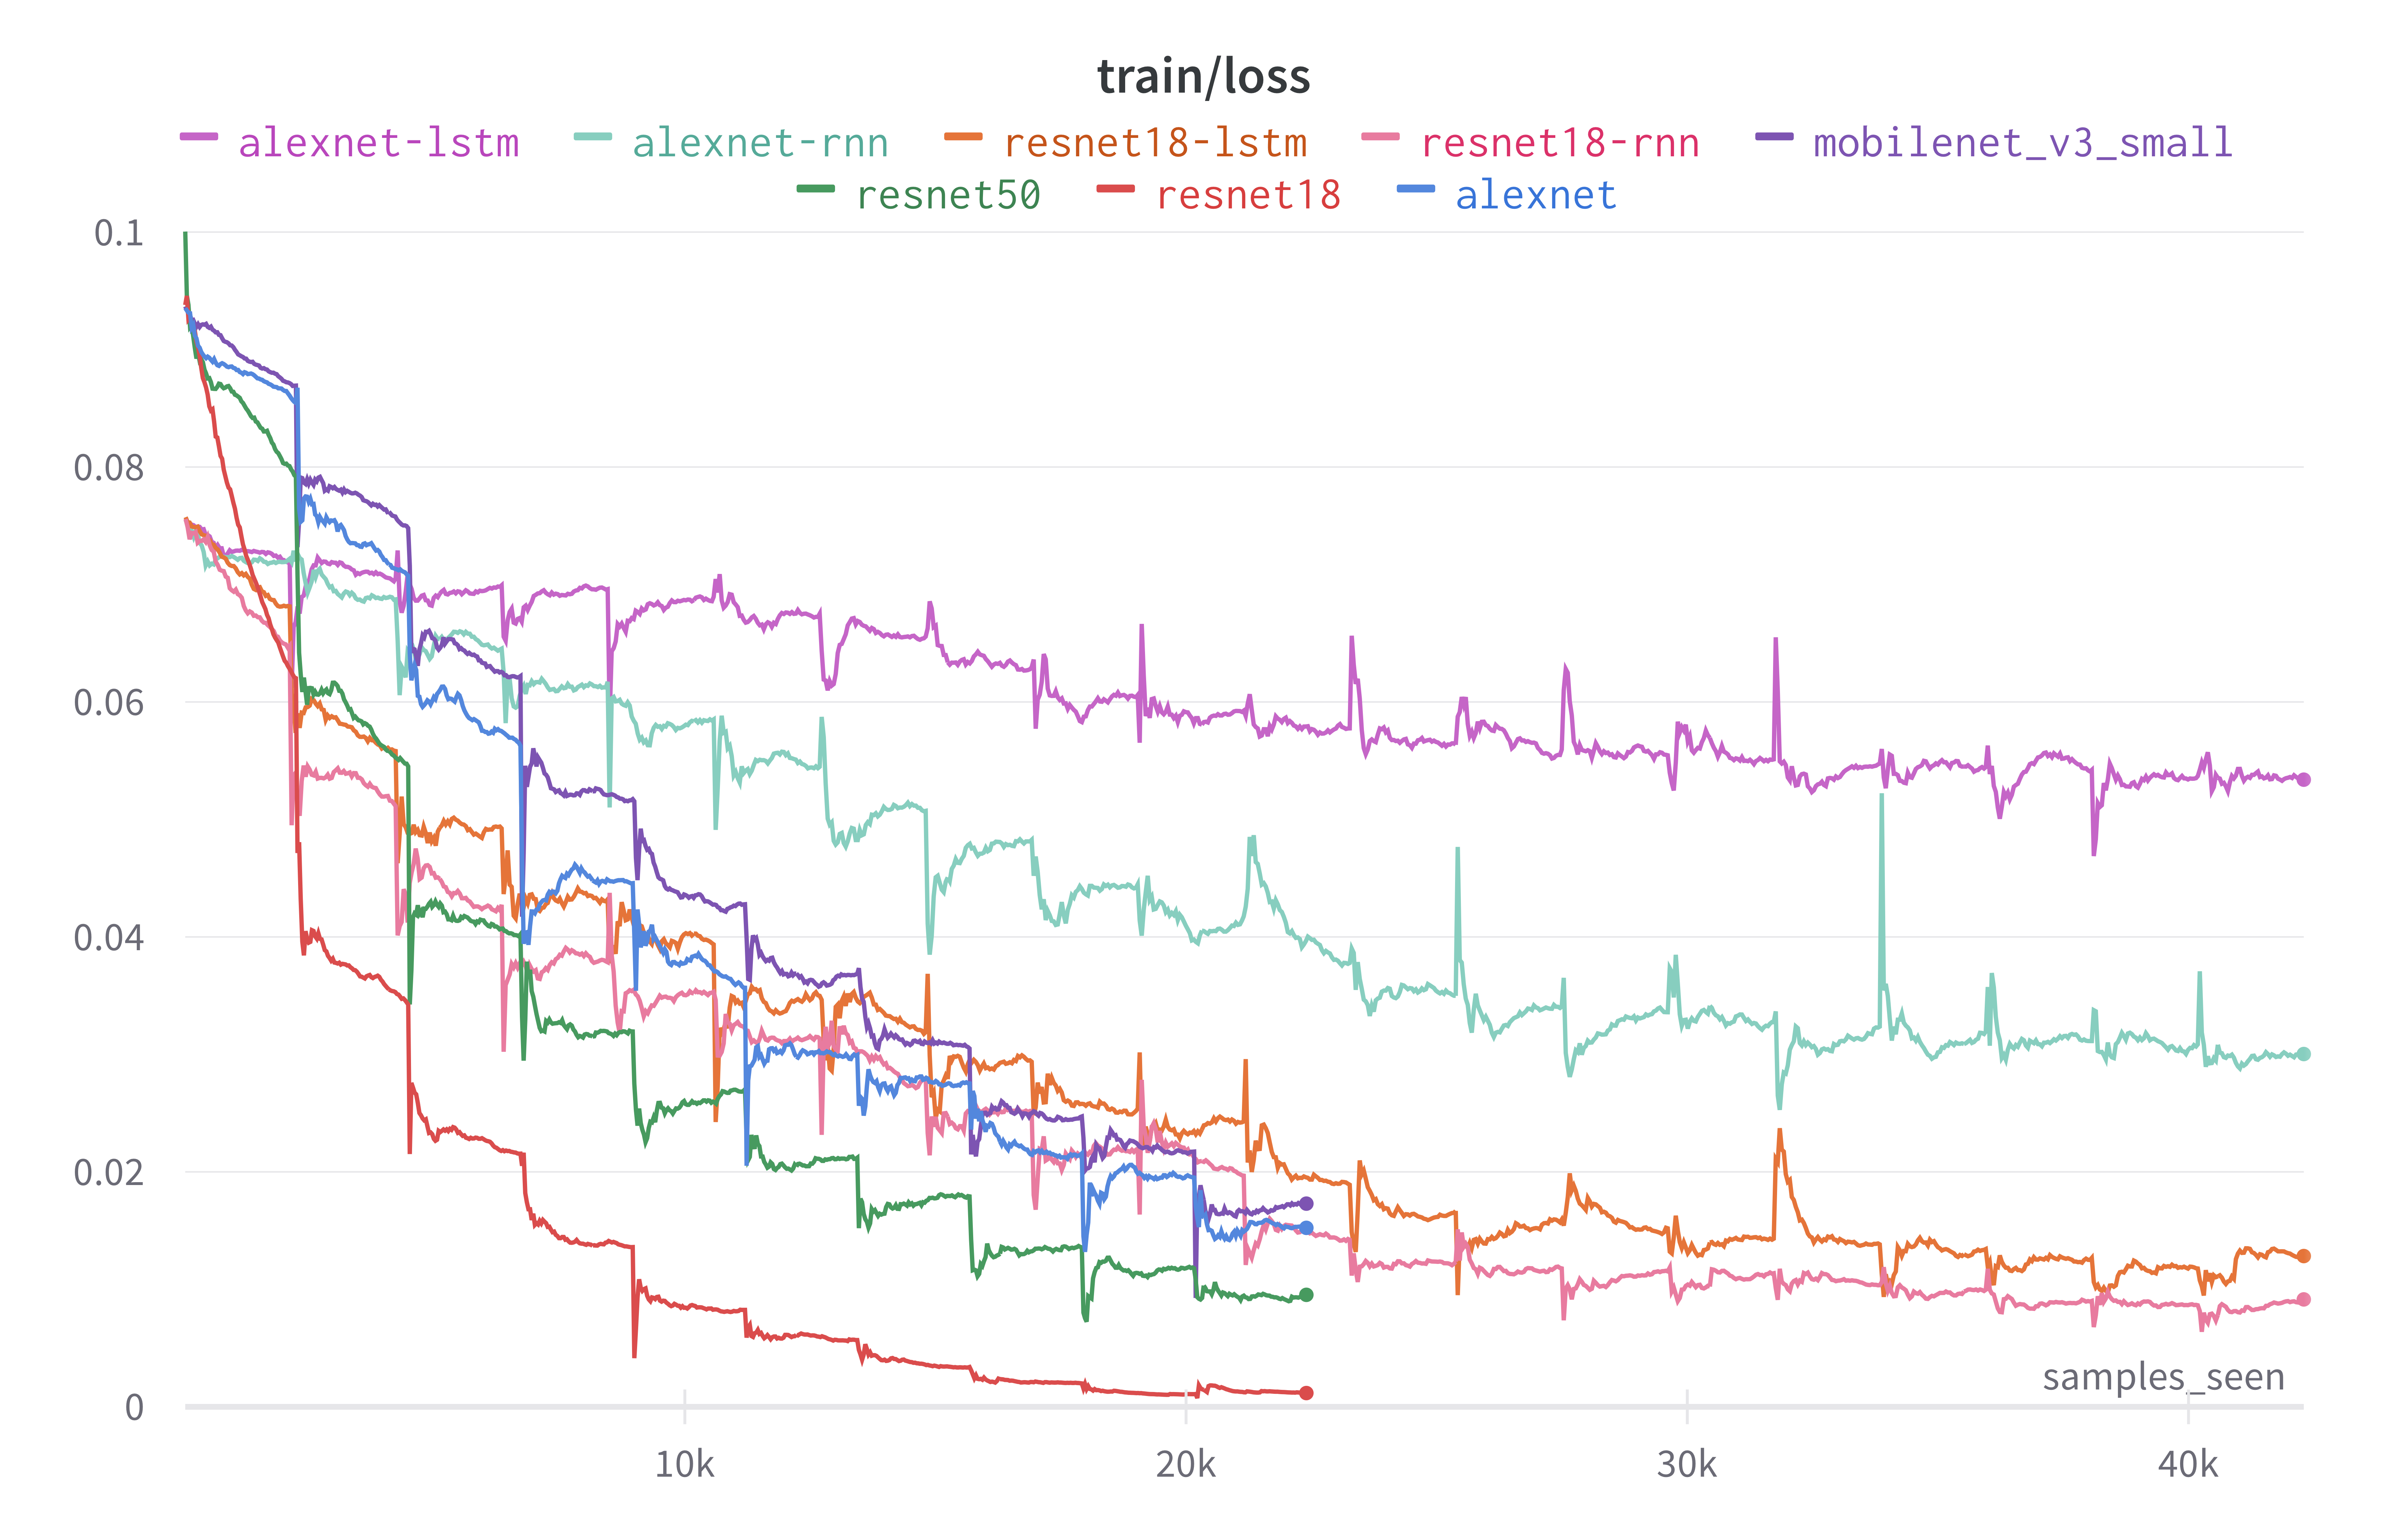
\includegraphics[width=\linewidth]{figures/experiment1-train-loss.png}
      \caption{Training Loss/ Samples}
      \label{fig:experiment1-train-acc}
    \end{subfigure}
    \hfill
    % subfigure
    \begin{subfigure}[b]{0.49\linewidth}
      \centering
      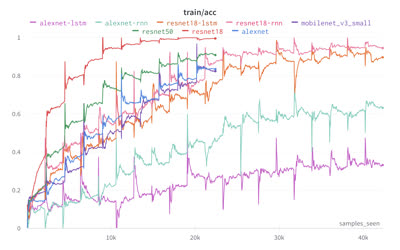
\includegraphics[width=\linewidth]{figures/experiment1-train-acc.jpg}
      \caption{Training Accuracy/ Samples}
      \label{fig:experiment1-train-loss}
    \end{subfigure}
    \caption{Training Metrics for Experiment 1}
    \label{fig:experiment-1-training}
  \end{figure}

  % encoding 
  \begin{table}[ht]
    \centering
    \begin{tabular}{lc}
    \toprule
    \bfseries Class & \bfseries Encoding \\
    \midrule
    First\_Floor\_Corridor\_1 & A \\
    First\_Floor\_Corridor\_2 & B \\
    First\_Floor\_Green\_Area & C \\
    First\_Floor\_Library\_1 & D \\
    First\_Floor\_Library\_2 & E \\
    First\_Floor\_Library\_3 & F \\
    First\_Floor\_Magenta\_Area & G \\
    First\_Floor\_Mezzanine & H \\
    First\_Floor\_Red\_Area & I \\
    First\_Floor\_Yellow\_Area & J \\
    Ground\_Floor\_Atrium & K \\
    Ground\_Floor\_Corridor\_1 & L \\
    Ground\_Floor\_Corridor\_2 & M \\
    Ground\_Floor\_Entrance\_Magenta & N \\
    Ground\_Floor\_Entrance\_Yellow & O \\
    Ground\_Floor\_Green\_Area & P \\
    Ground\_Floor\_Magenta\_Area & Q \\
    Ground\_Floor\_Red\_Area & R \\
    Ground\_Floor\_Yellow\_Area & S \\
    Stairs\_Atrium & T \\
    \bottomrule
    \end{tabular}
    \caption{Encoding of Classes}
    \label{tab:class-encoding}
  \end{table}

  % figure
  \begin{figure}[ht]
    \centering
    % subfigure
    \begin{subfigure}[b]{0.49\linewidth}
      \centering
      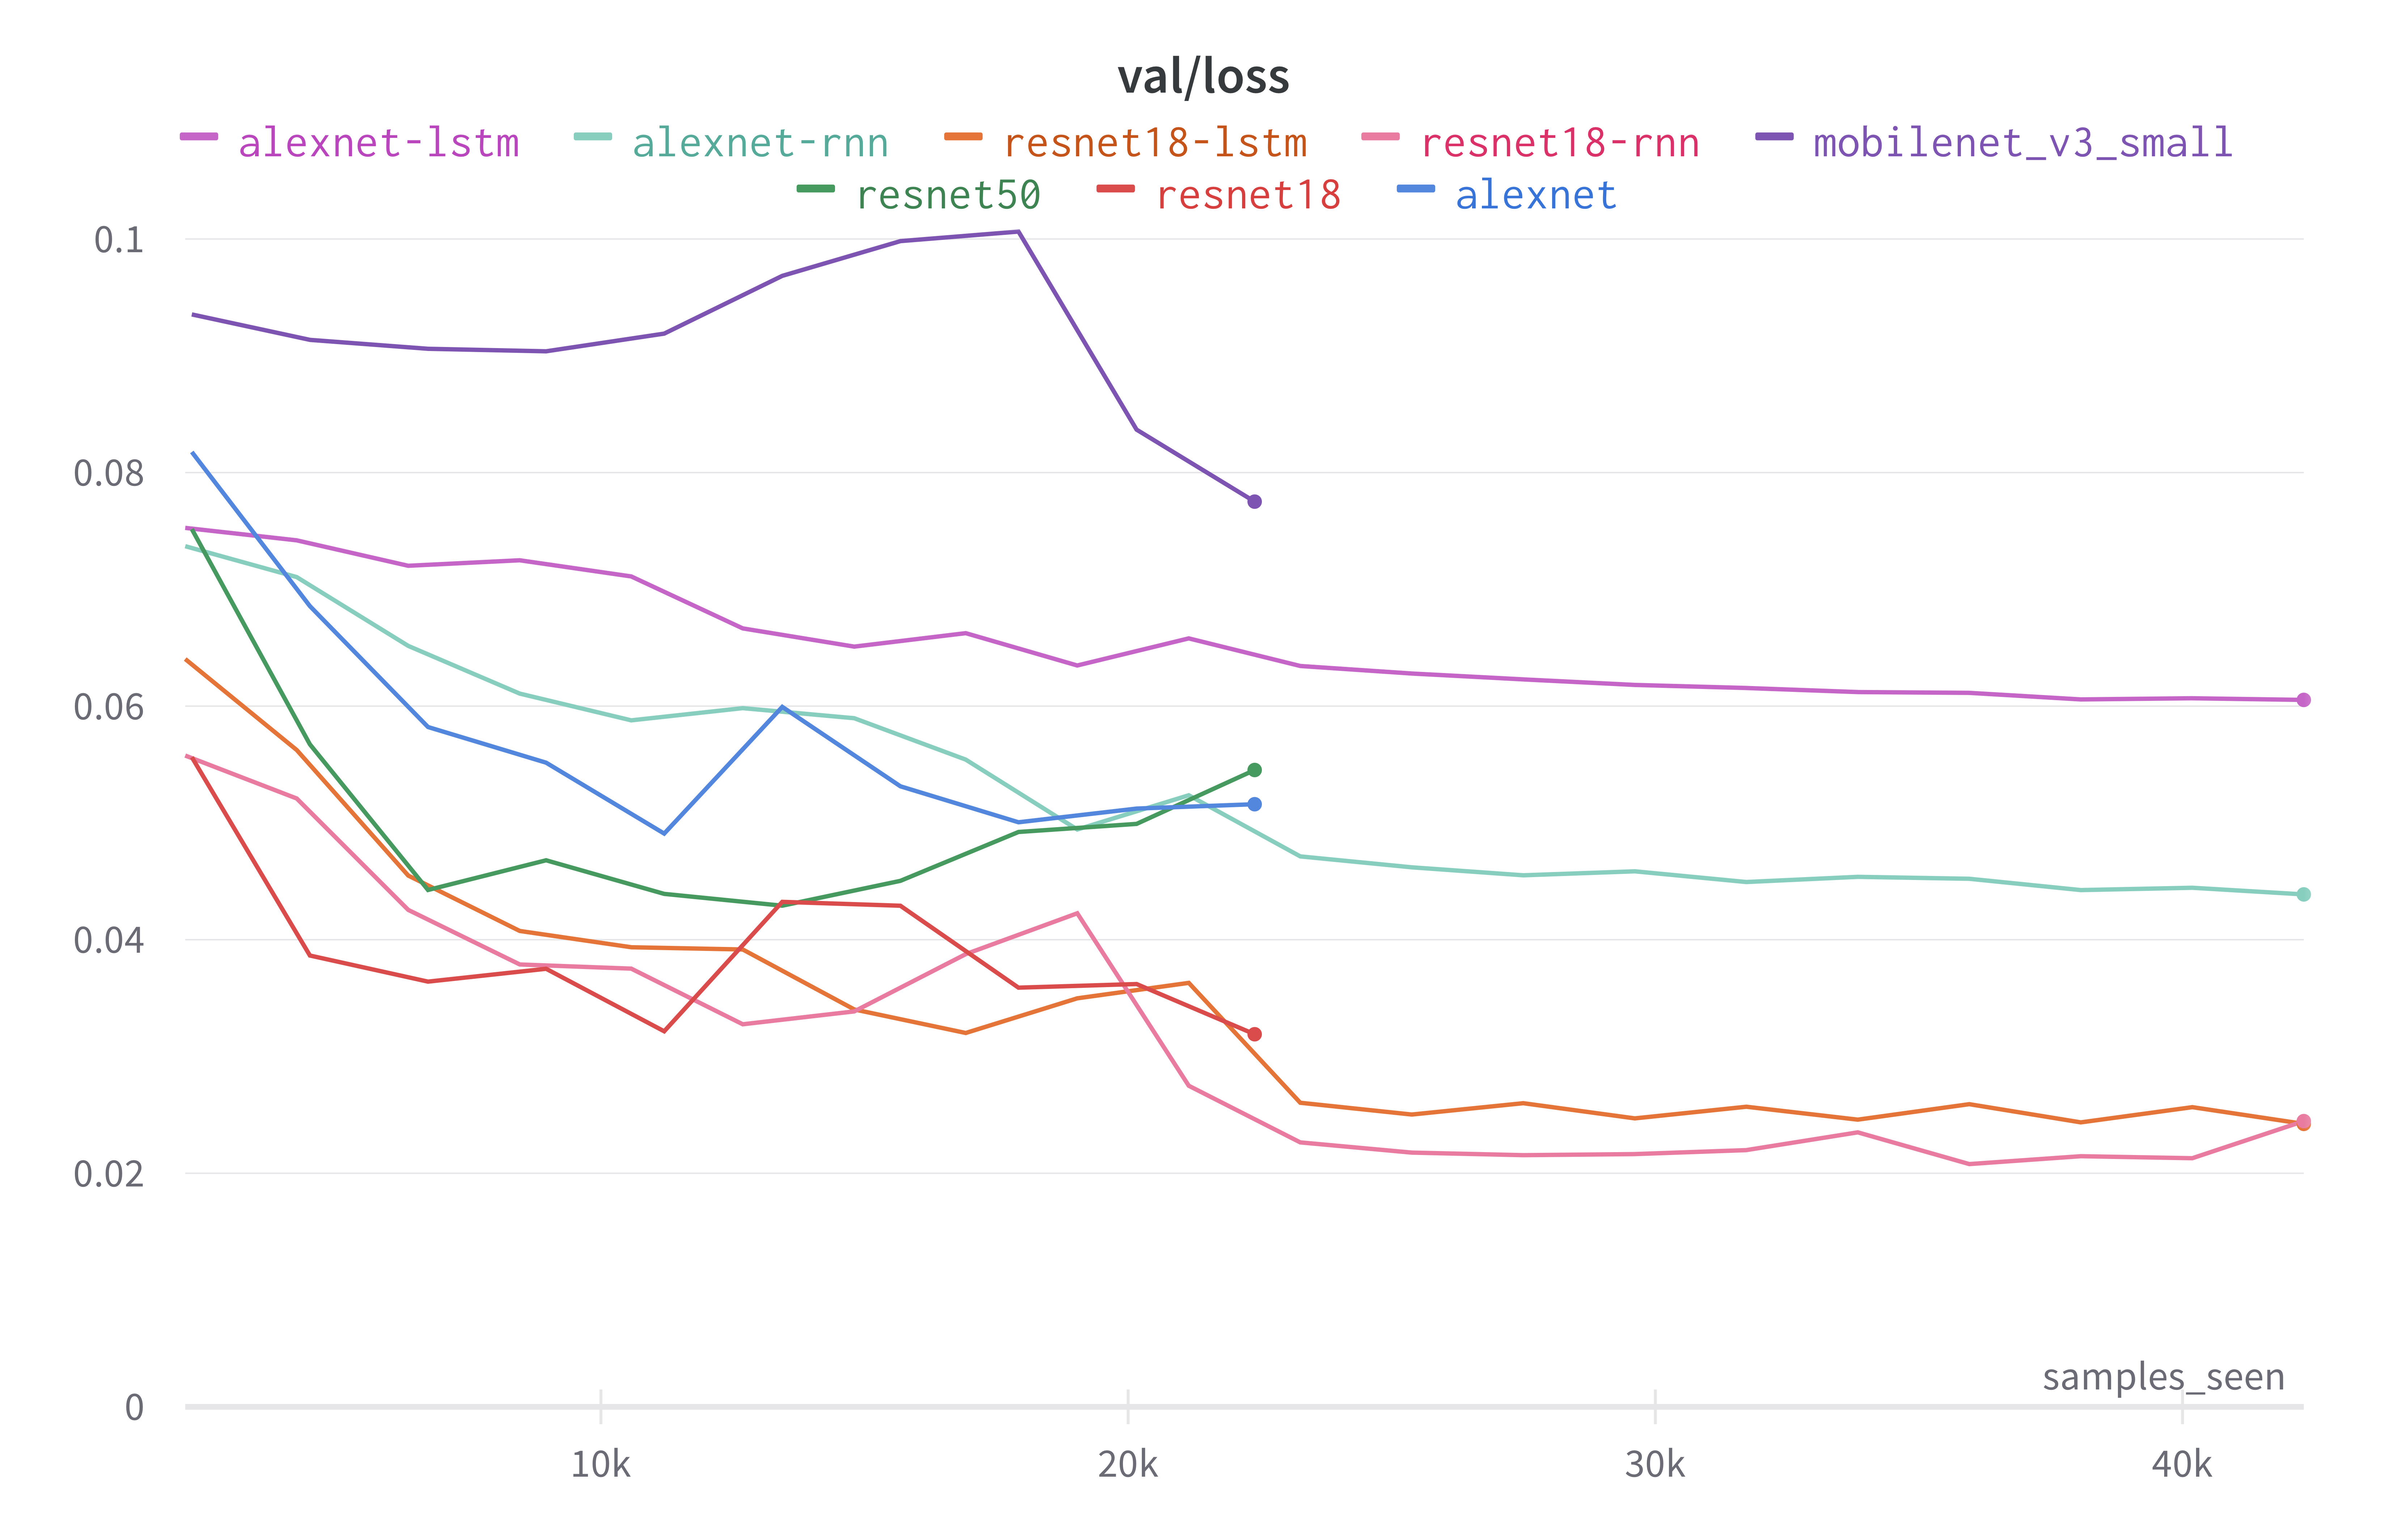
\includegraphics[width=\linewidth]{figures/experiment1-val-loss.png}
      \caption{Validation Loss/ Samples}
      \label{fig:experiment1-val-acc}
    \end{subfigure}
    \hfill
    % subfigure
    \begin{subfigure}[b]{0.49\linewidth}
      \centering
      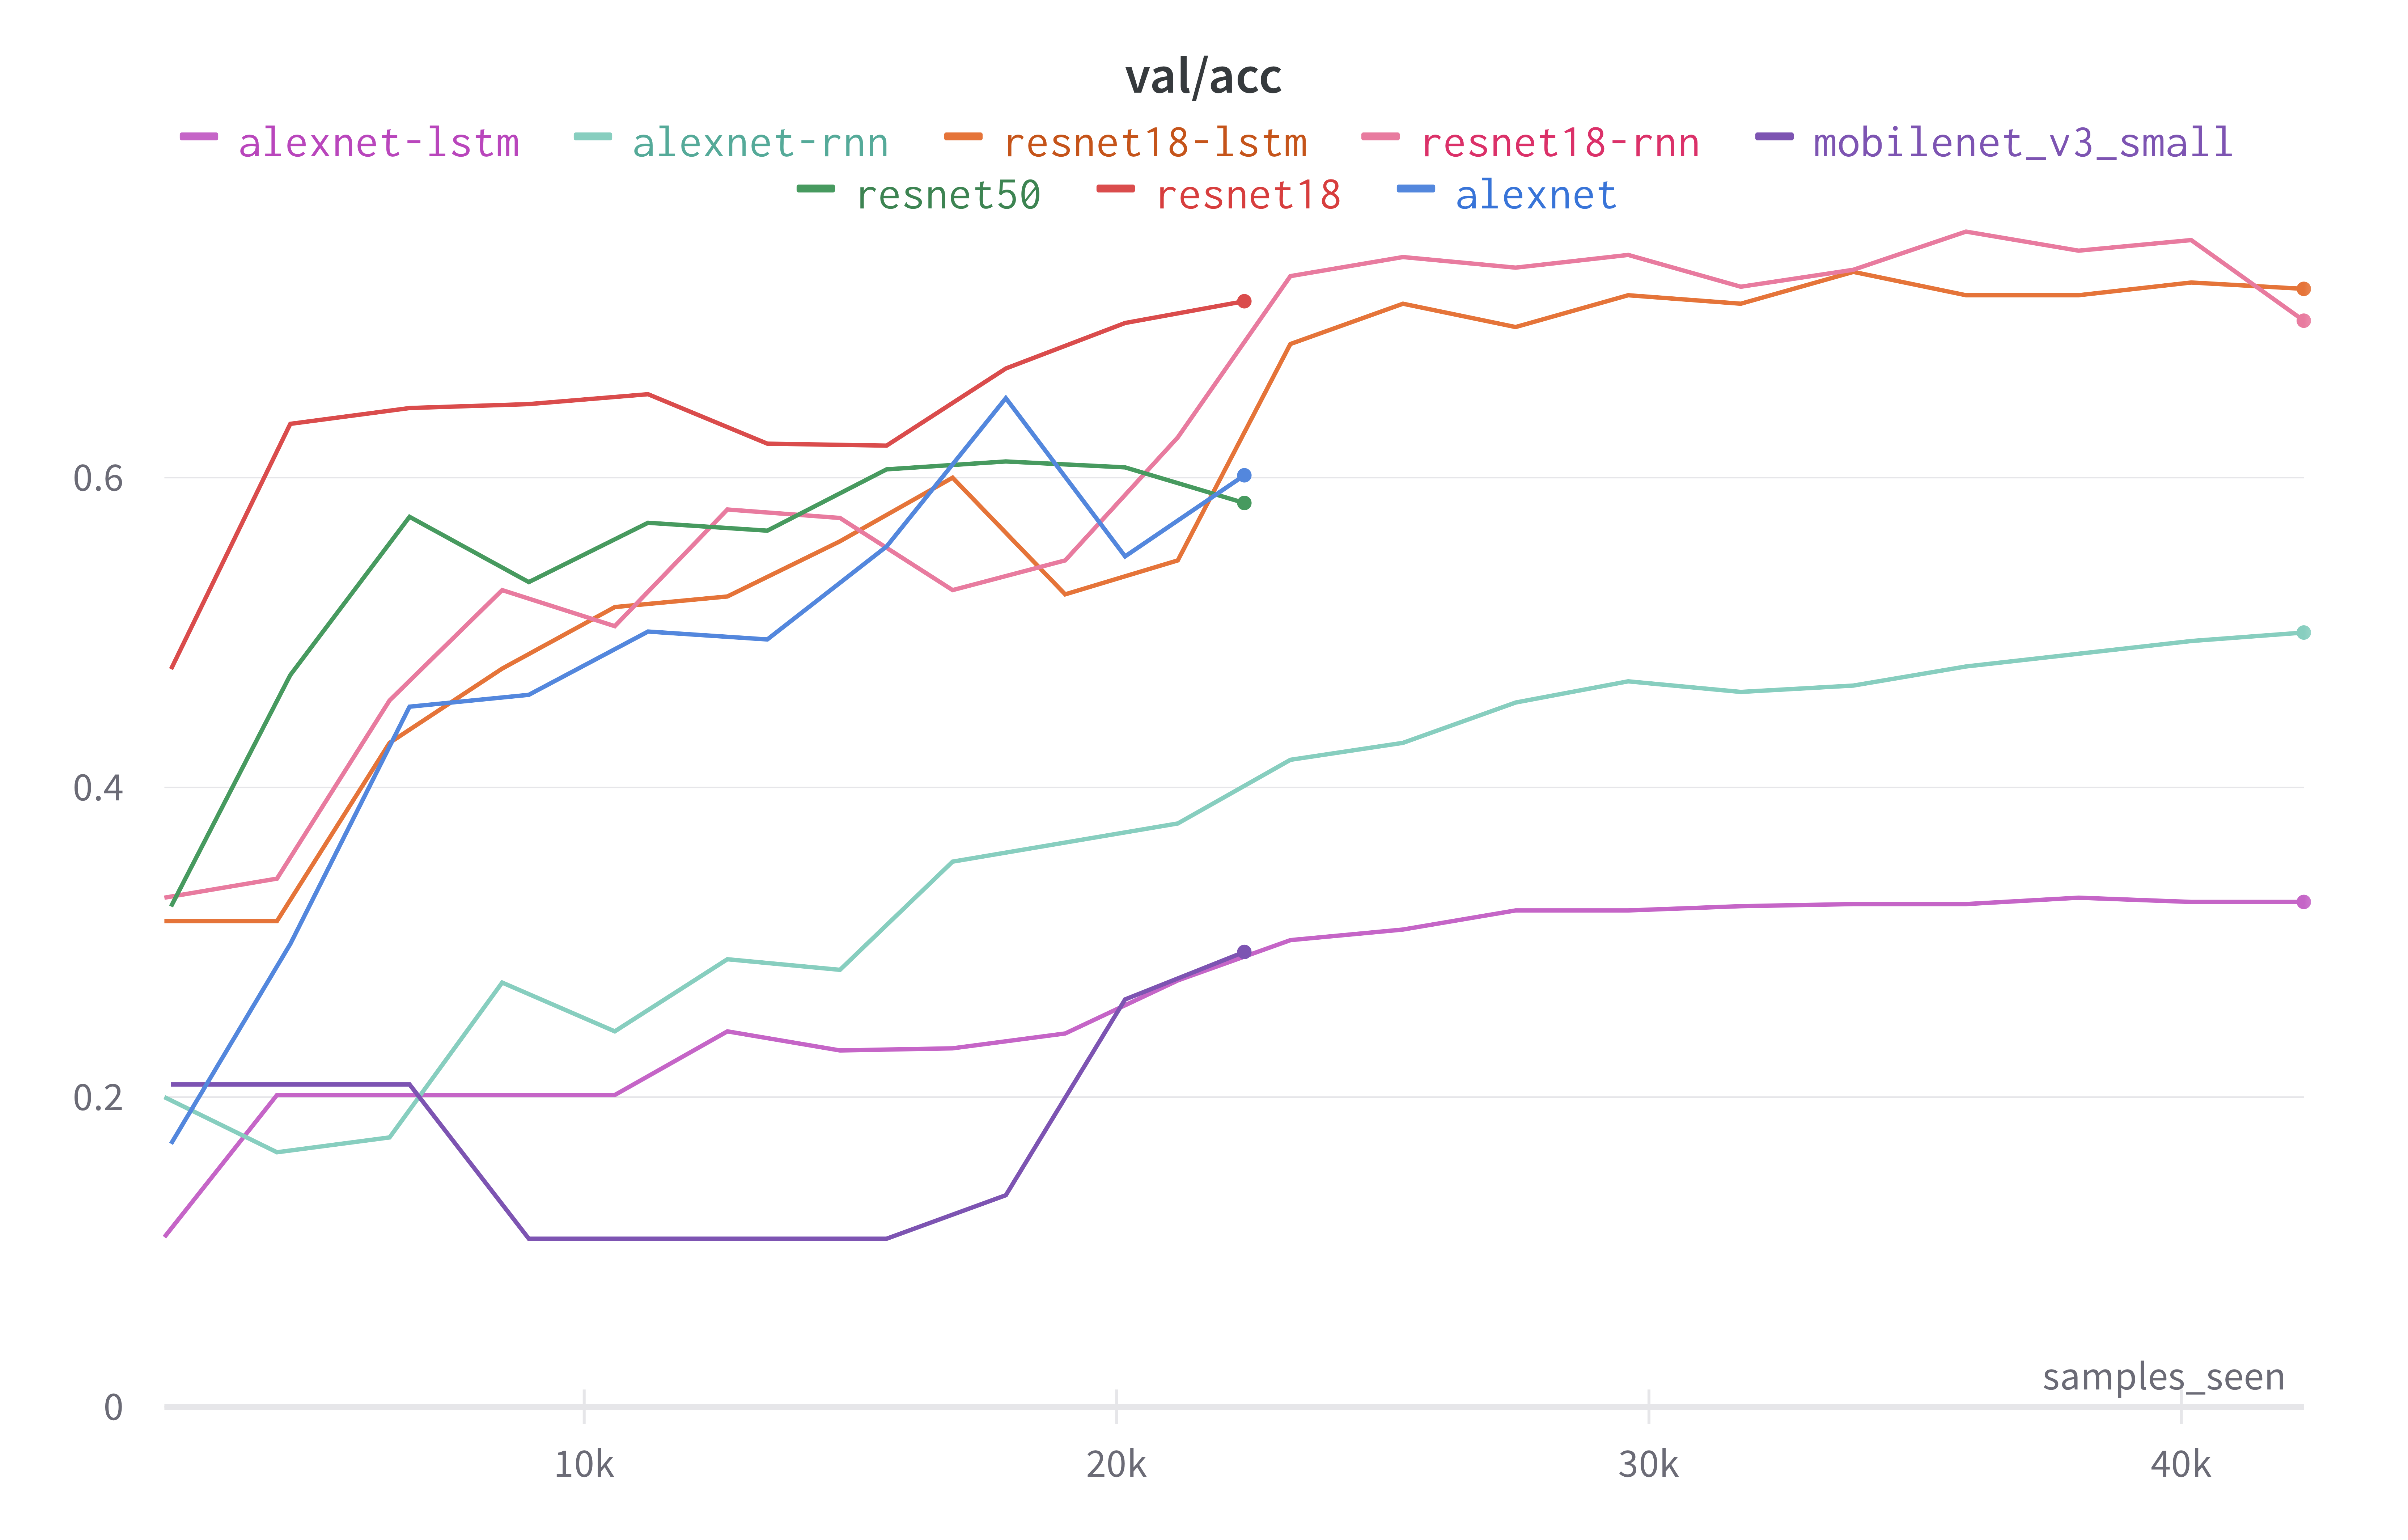
\includegraphics[width=\linewidth]{figures/experiment1-val-acc.png}
      \caption{Valiation Accuracy/ Samples}
      \label{fig:experiment1-val-loss}
    \end{subfigure}
    \caption{Validation Metrics for Experiment 1}
    \label{fig:experiment-1-validation}
  \end{figure}


  \begin{table}[ht]
    \centering
    \begin{tabular}{clllllll}
      \toprule
      & \multirow{2}{*}{\textbf{Model}} 
      & \textbf{1-Acc.} & \textbf{3-Acc.}& \textbf{Ma.-F1} & \textbf{Par.} & \textbf{FLOPs} & \textbf{Throughput} \\
      & & (\%) & (\%) & (\%) & (M) & (G) & (Preds/s) \\
      \midrule
    \multirow{4}{*}{\rotatebox[origin=c]{90}{Image}} &
        \texttt{alexnet} & 60.15 & 84.42 & 55.95 & 57.09 & 0.71 & \bfseries
        87.31 ($\pm$ 1.15) \\
      & \texttt{resnet18} & 71.39 & 91.70 & \bfseries 68.29 & 11.19 & 1.82 &
      64.12 ($\pm$ 1.90) \\
      & \texttt{resnet50} & 58.37 & 82.63 & 55.92 & 23.55 & 4.12 & 27.57 ($\pm$ 1.10) \\
      & \texttt{mobilenet\_v3} & 29.37 & 64.11 & 14.87 & 1.54 & 0.06 &
      16.49 ($\pm$ 1.44) \\

      \midrule

      \multirow{4}{*}{\rotatebox[origin=c]{90}{Video}}
      & \texttt{alexnet-lstm} & 32.60 & 62.19 & 9.95 & \bfseries 58.58 & 3.57 &
      38.31 ($\pm$ 0.53) \\
      & \texttt{alexnet-rnn} & 50.00 & 78.90 & 35.71 & 58.19 & 3.56 & 39.09
      ($\pm$ 0.51) \\
      & \texttt{resnet18-lstm} & \bfseries 72.19 & 91.78 & 64.59 & 11.84 &
        \bfseries 9.11 & 19.66 ($\pm$ 0.40) \\
      & \texttt{resnet18-rnn} & 70.14 & \bfseries 93.97 & 66.62 & 11.44 & 9.11 &
      19.07 ($\pm$ 0.56) \\

      \bottomrule
    \end{tabular}
    \caption{Results of Experiment 1}
    \label{tab:results-experiment1}
  \end{table}

  % section Results (end)

  \section{Limitations \& Future Work} % (fold)
  \label{sec:discussion}

  % section Discussion (end)

  \section{Conclusion} % (fold)
  \label{sec:conclusion}

  We have shown that the problem of indoor localisation can be phrased as a
  classification problem and be solved through the use of deep learning models
  in a data-efficient manner.
  Simple convolutional neural architectures were able to provide accurate and
  robust predictions and showed emerging learning of features mostly invariant
  to natural variations in the environment.
  The use of a recurrent neural network architecture allowed for the
  incorporation of temporal information and improved the accuracy of the
  predictions, though only marginally so.

  % section Conclusion (end)

  \section{Remarks} % (fold)
  \label{sec:remarks}

  \subsection{Reproducibility} % (fold)
  \label{sub:reproducibility}

  All code and data used in this project is available on GitHub at the
  following link: \url{https://github.com/mikasenghaas/bsc}. The project's 
  \texttt{README} file contains detailed instructions on how to reproduce the
  results of this project.

  Further, the precise configuration and results of the experiments that are
  reported here are publicly available on the Weights \& Biases platform at the
  following link: \url{https://wandb.ai/mikasenghaas/bsc}.

  % subsection reproducibility (end)

  \subsection{Machine Specifications} % (fold)
  \label{sub:machine-specs}

  Table~\ref{tab:machine-specs} lists the specifications of the machine that was
  used for training and evaluation of the models. For training the \texttt{MPS}
  backend was used for accelerated training. However, for inference a single CPU
  core was used, to approximate latency and throughput on mobile devices.


  \begin{table}[ht]
    \centering
    \begin{tabular}{cll}
     \toprule
     & Specification & Value \\
     \midrule

     \multirow{2}{*}{System} & Name & Darwin \\
     \vspace{0.1cm}
     & Node & Local MacBook Pro \\

     \multirow{4}{*}{CPU} & Model & Apple M1 \\
     & Architecture & ARM64 \\
     & Physical Cores & 8 \\
     \vspace{0.1cm}
     & Frequency & 2.4 GHz \\

     \multirow{2}{*}{Memory} & Total Capacity & 16 GB \\
     & Avg. Used Capacity & $\sim 7.4$ GB \\

     \bottomrule
    \end{tabular}
    \caption{Machine Specifications}
    \label{tab:machine-specs}
  \end{table}
  
  % subsection subsection name (end)

  % section remarks (end)

  % bibliography
  \newpage
  \bibliography{references}
  \bibliographystyle{plain}

  \section{Appendix} % (fold)
  \label{sec:appendix}

  % conf matrices for all models
  \newgeometry{margin=1cm}
  \begin{figure}[b]
    \centering
    \begin{subfigure}{.33\textwidth}
        \centering
        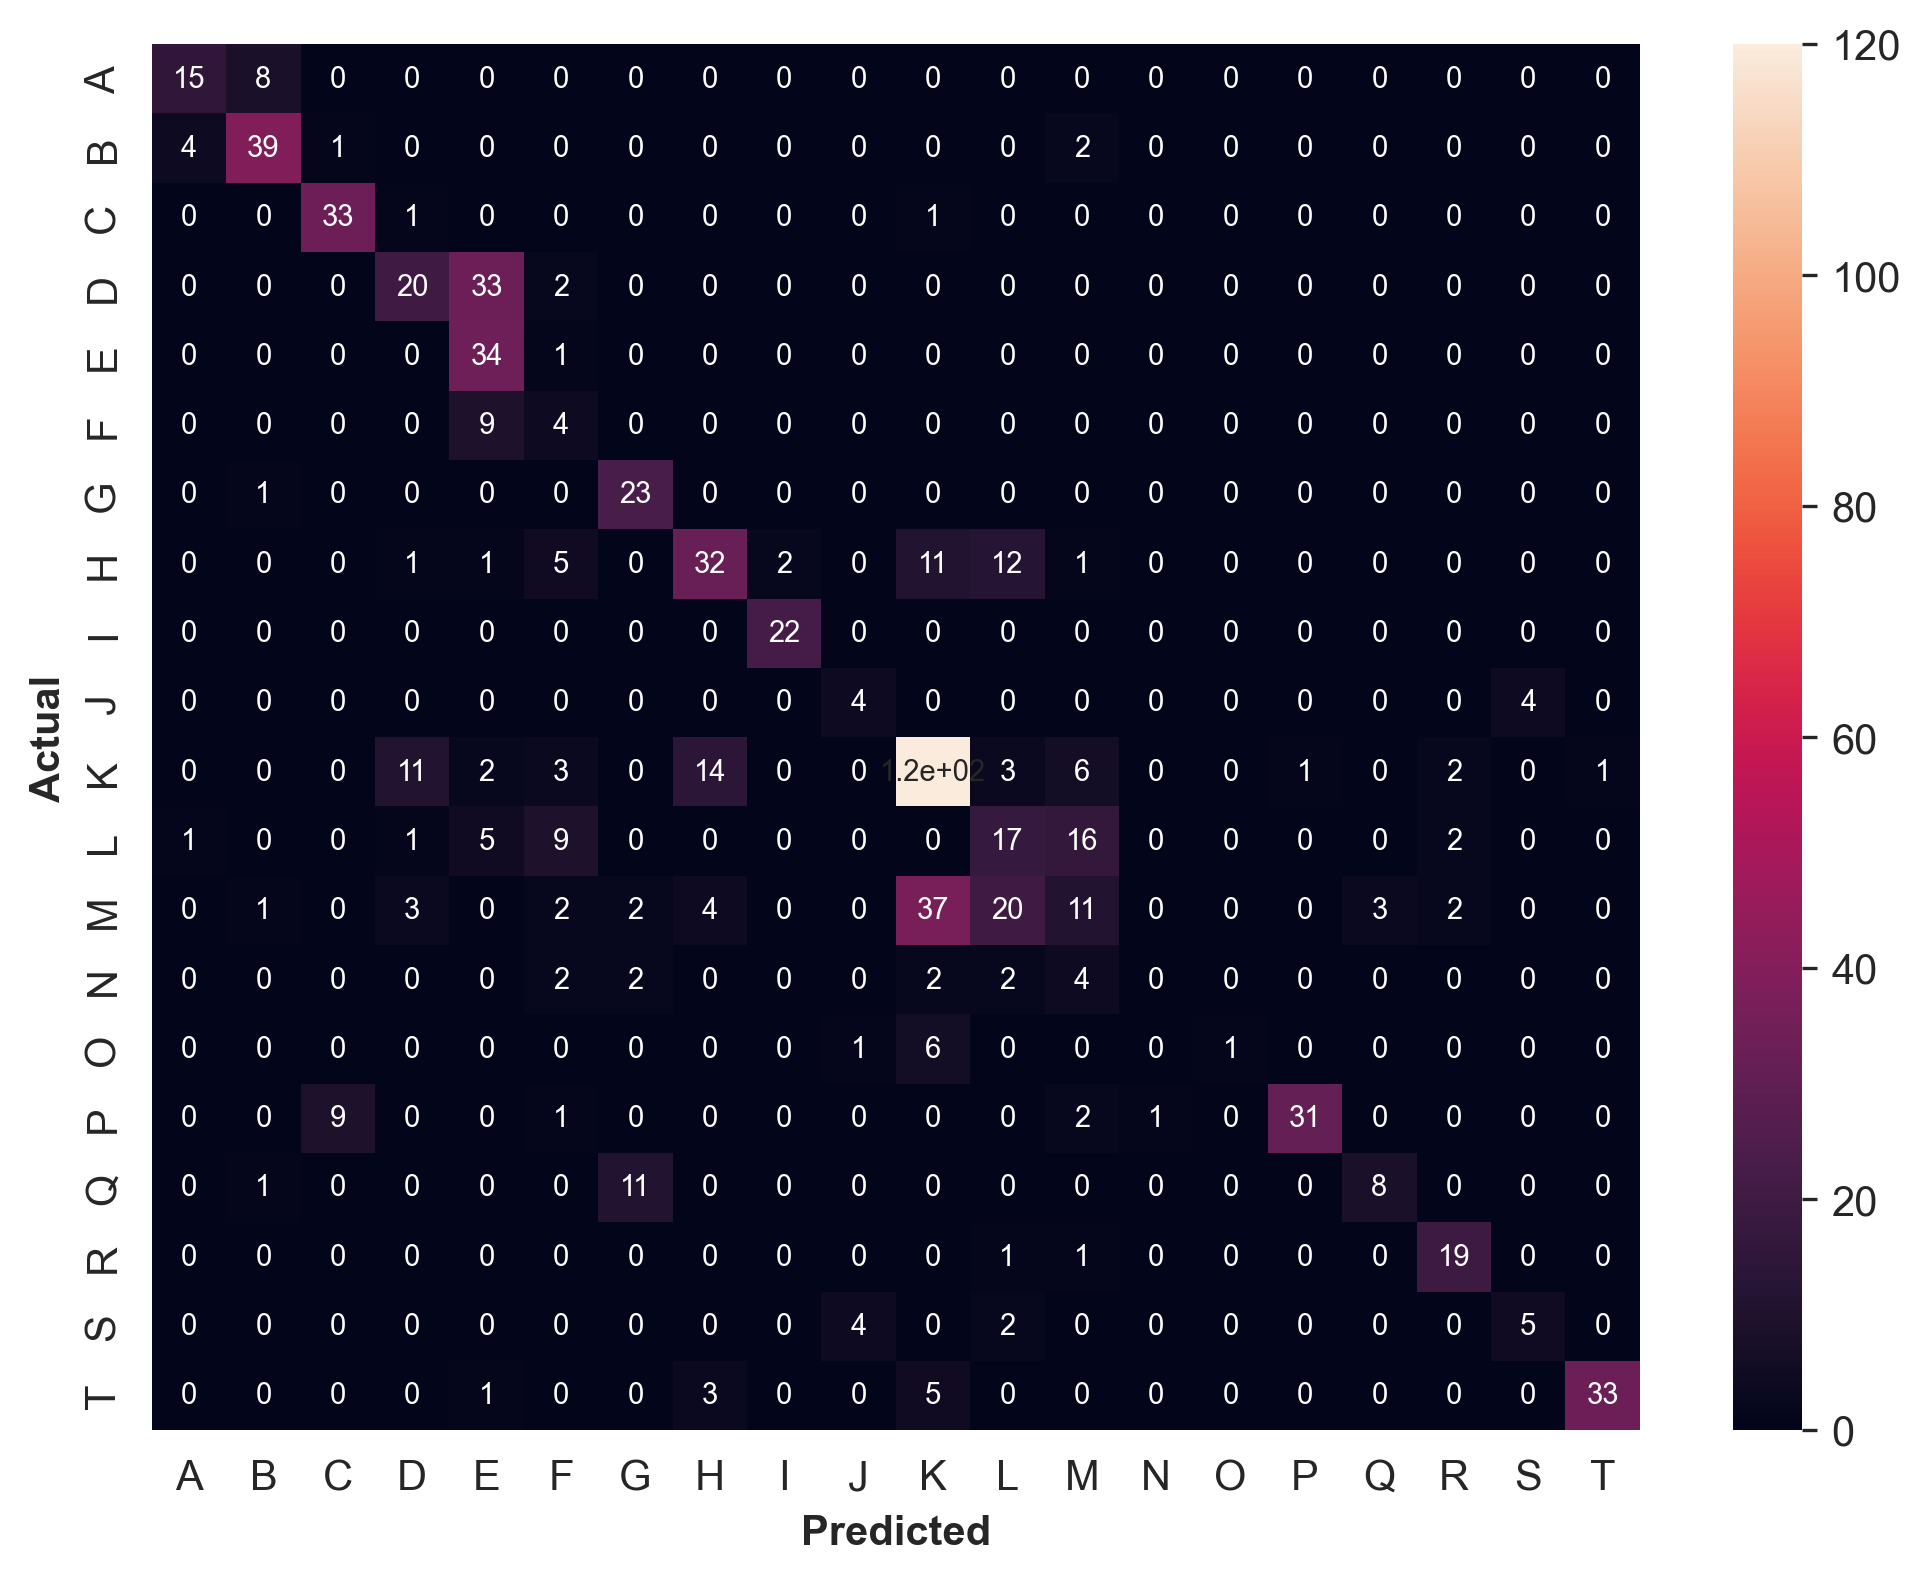
\includegraphics[width=\textwidth]
        {figures/experiment1-conf-matrix-alexnet.png}
        \caption{\texttt{alexnet}}
    \end{subfigure}%
    \begin{subfigure}{.33\textwidth}
        \centering
        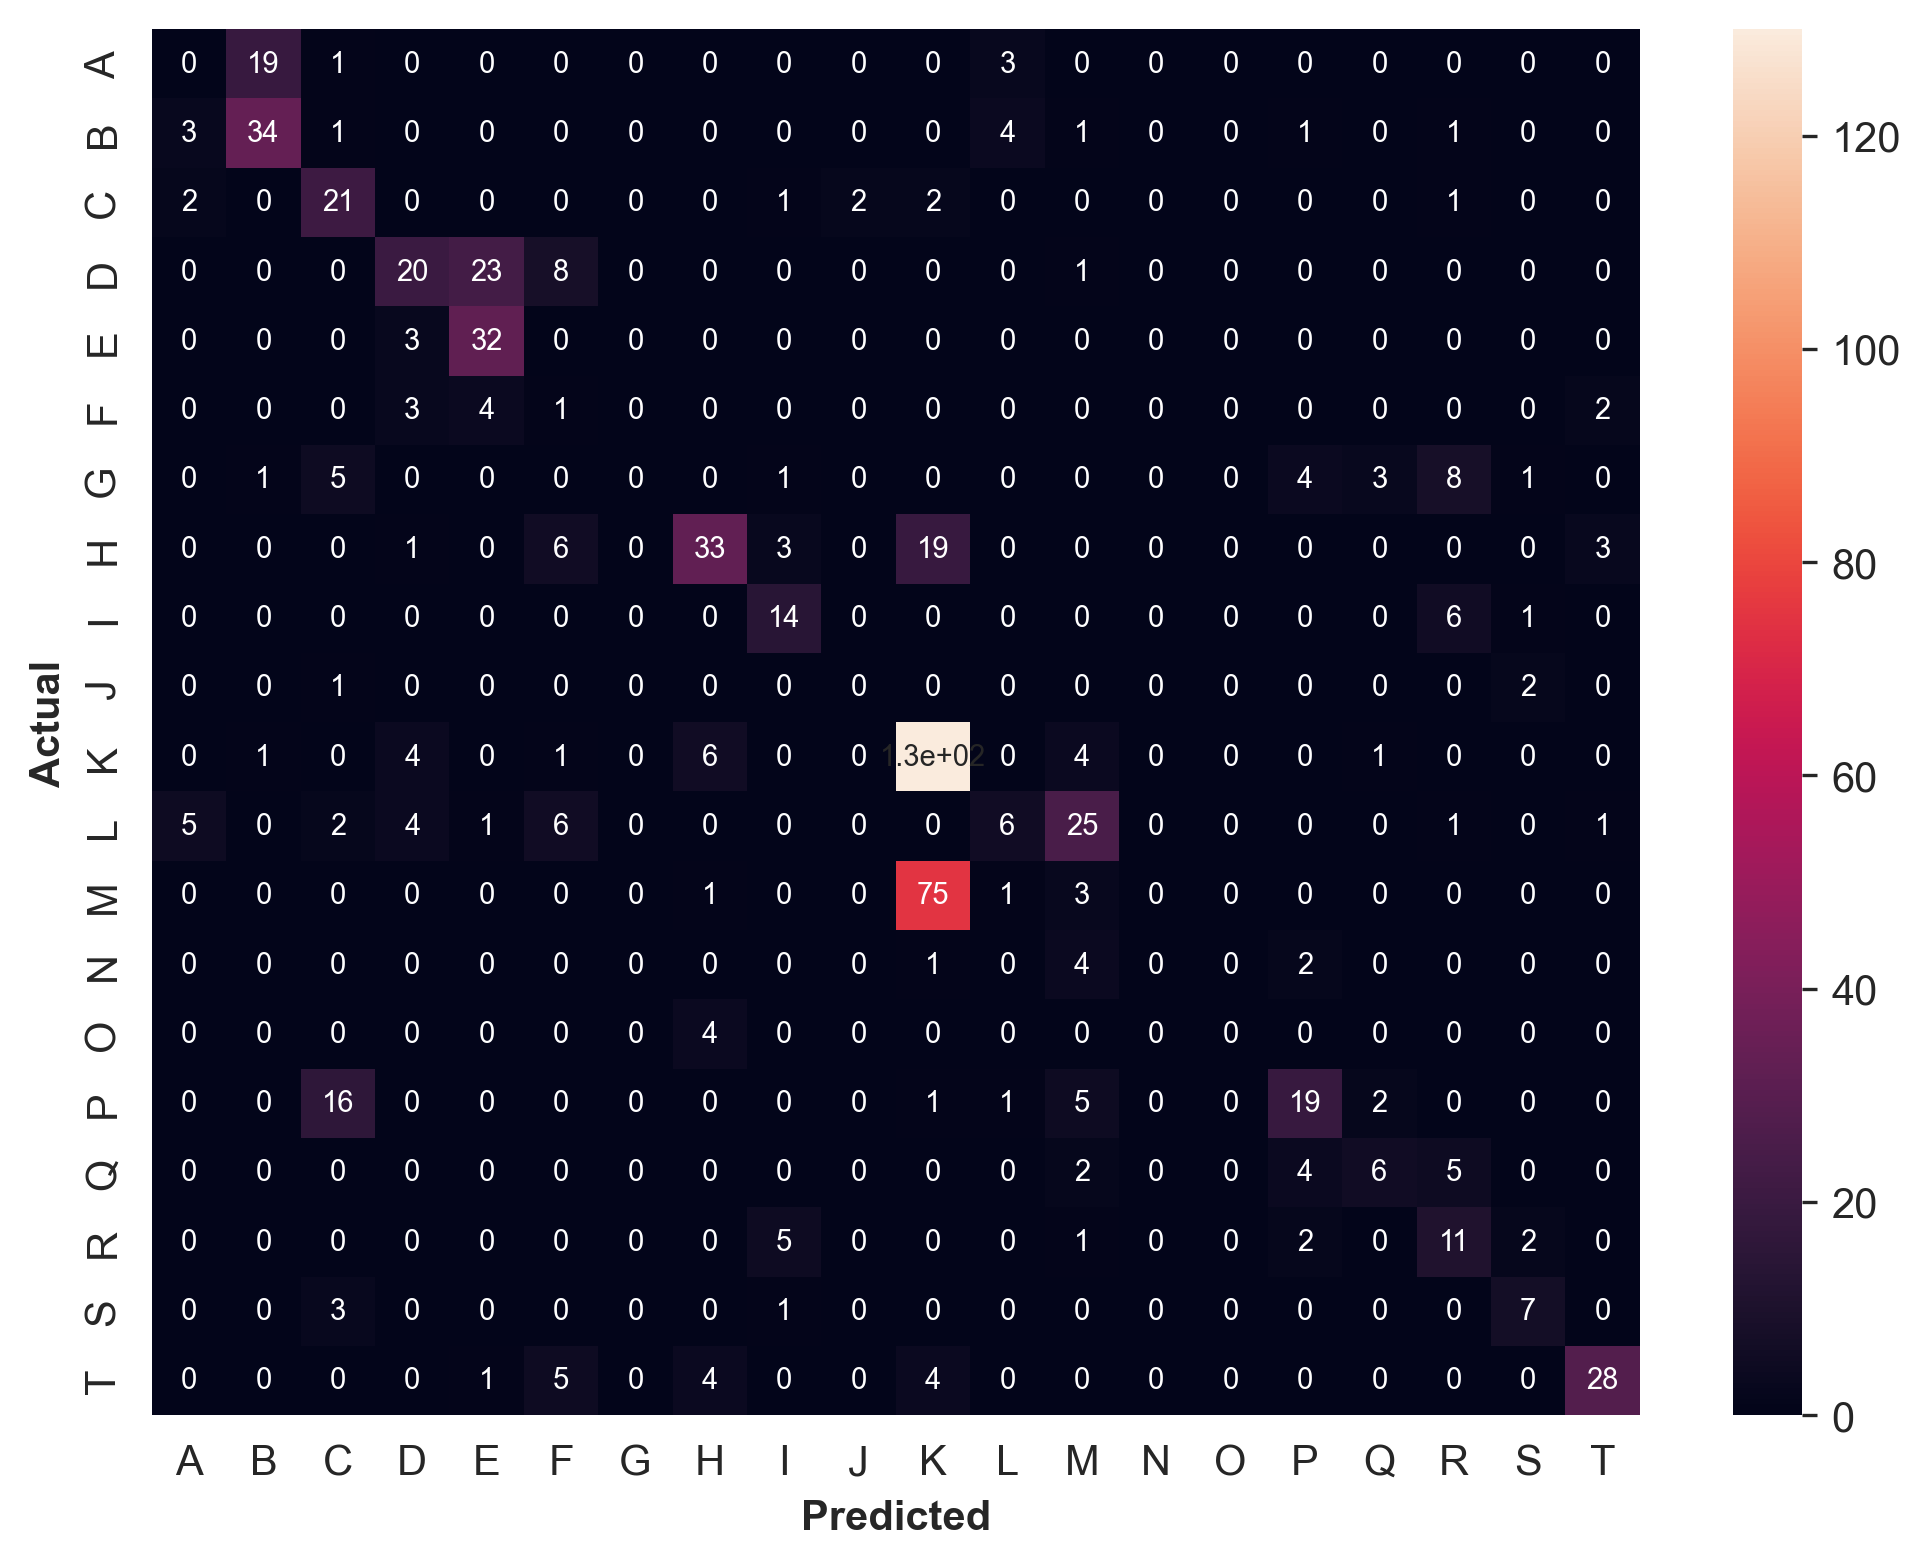
\includegraphics[width=\textwidth]
        {figures/experiment1-conf-matrix-alexnet-rnn.png}
        \caption{\texttt{alexnet-rnn}}
    \end{subfigure}
    \begin{subfigure}{.33\textwidth}
        \centering
        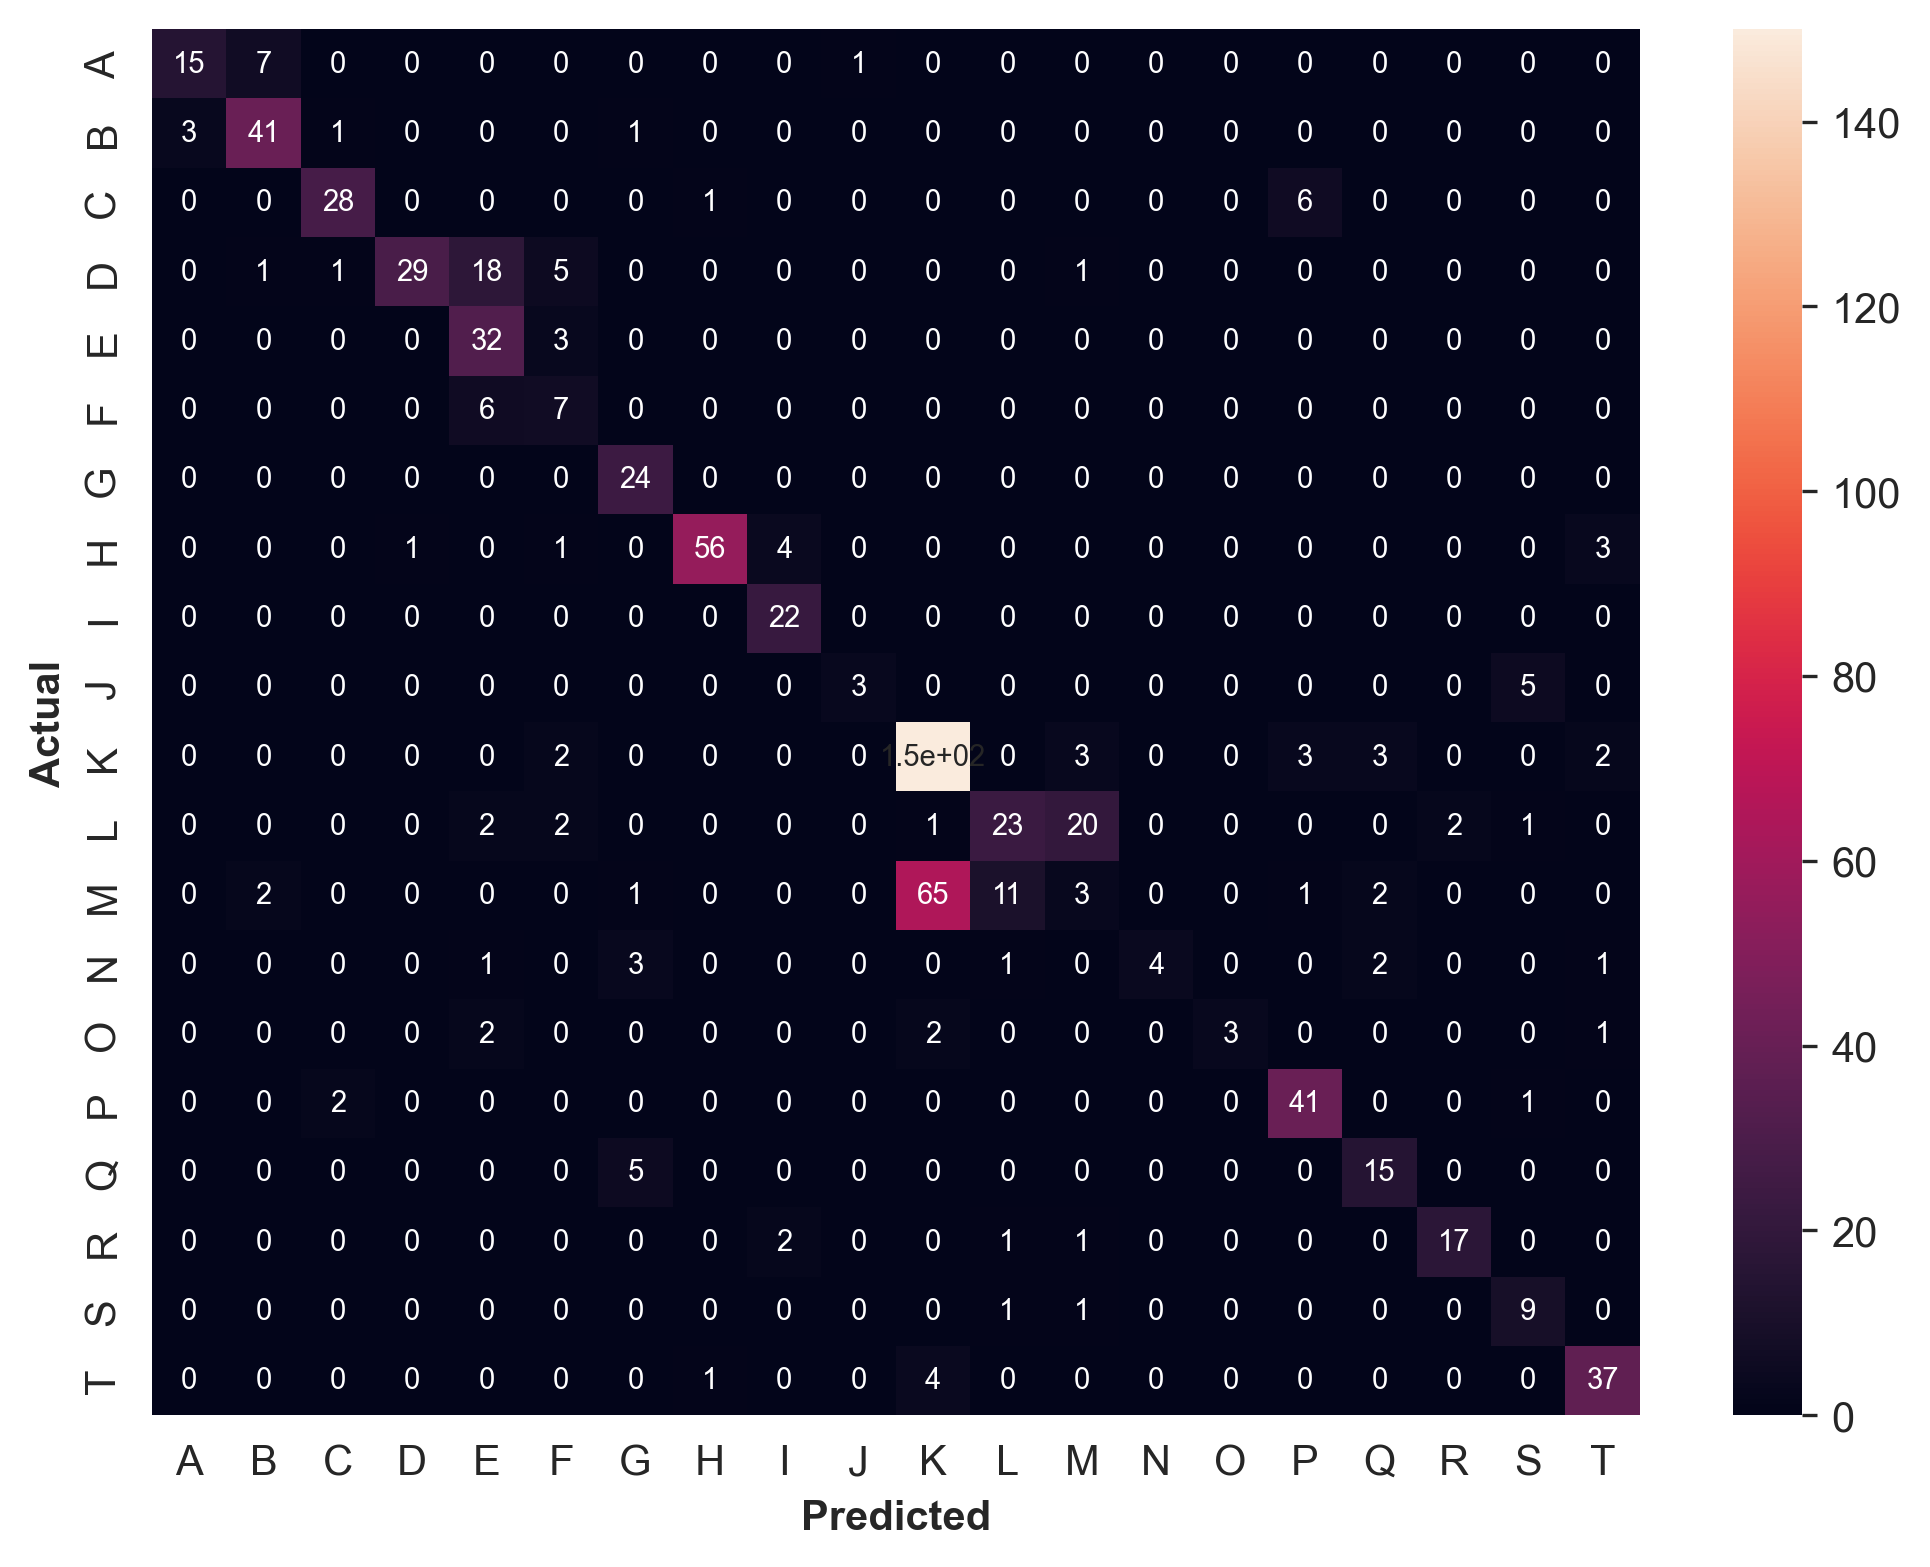
\includegraphics[width=\textwidth]
        {figures/experiment1-conf-matrix-resnet18.png}
        \caption{\texttt{resnet18}}
    \end{subfigure}
    \begin{subfigure}{.33\textwidth}
        \centering
        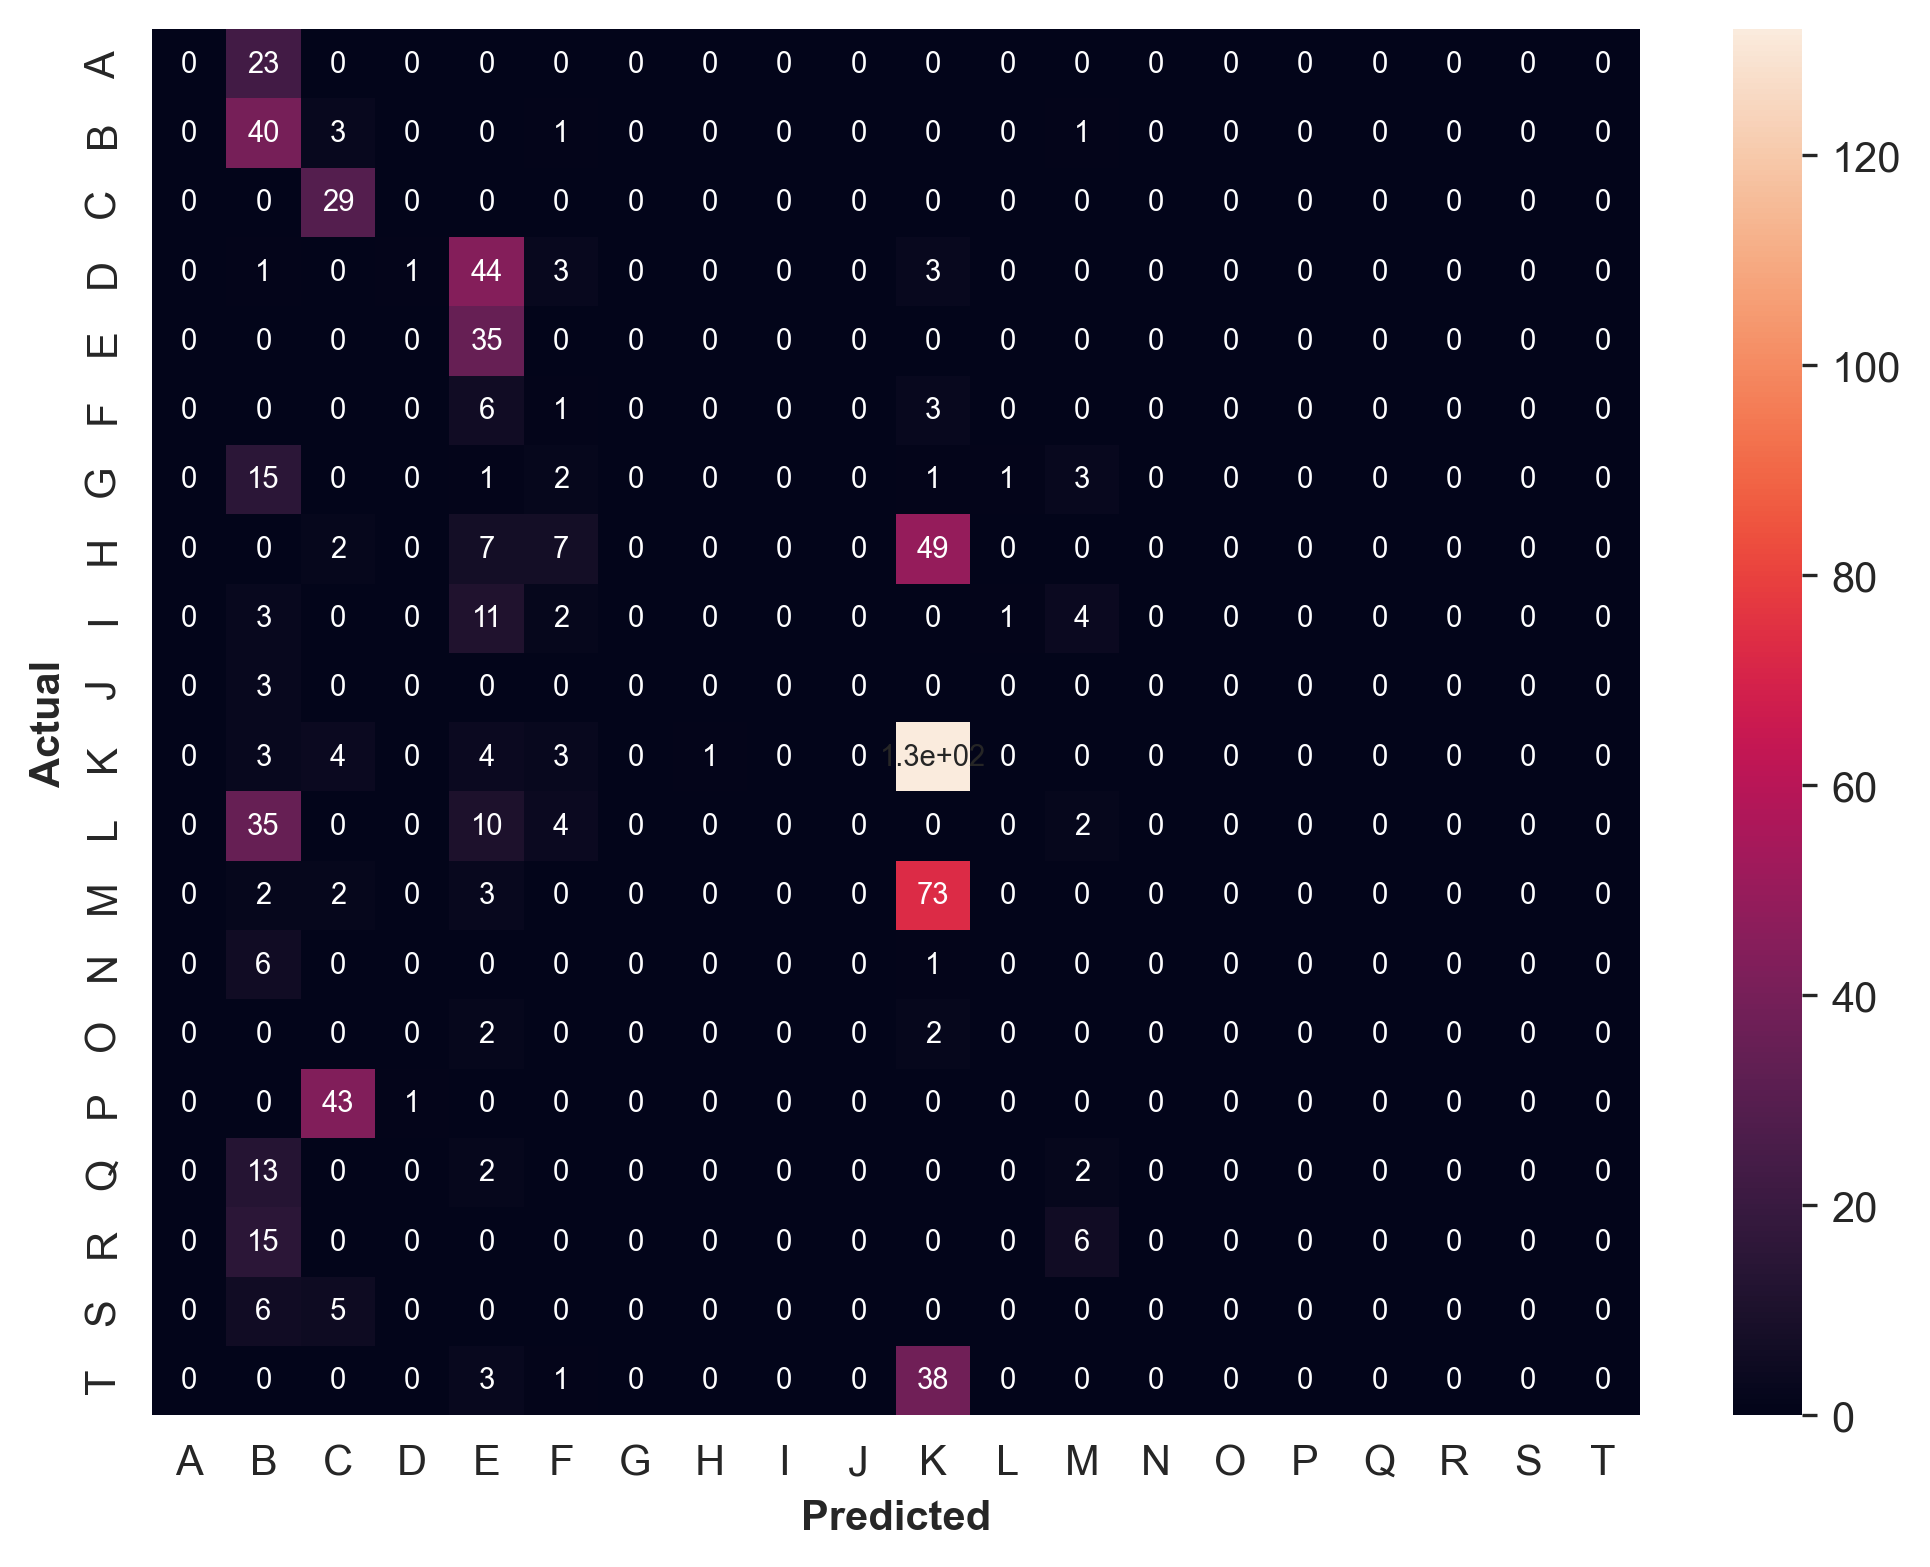
\includegraphics[width=\textwidth]
        {figures/experiment1-conf-matrix-alexnet-lstm.png}
        \caption{\texttt{alexnet-lstm}}
    \end{subfigure}
    \begin{subfigure}{.33\textwidth}
        \centering
        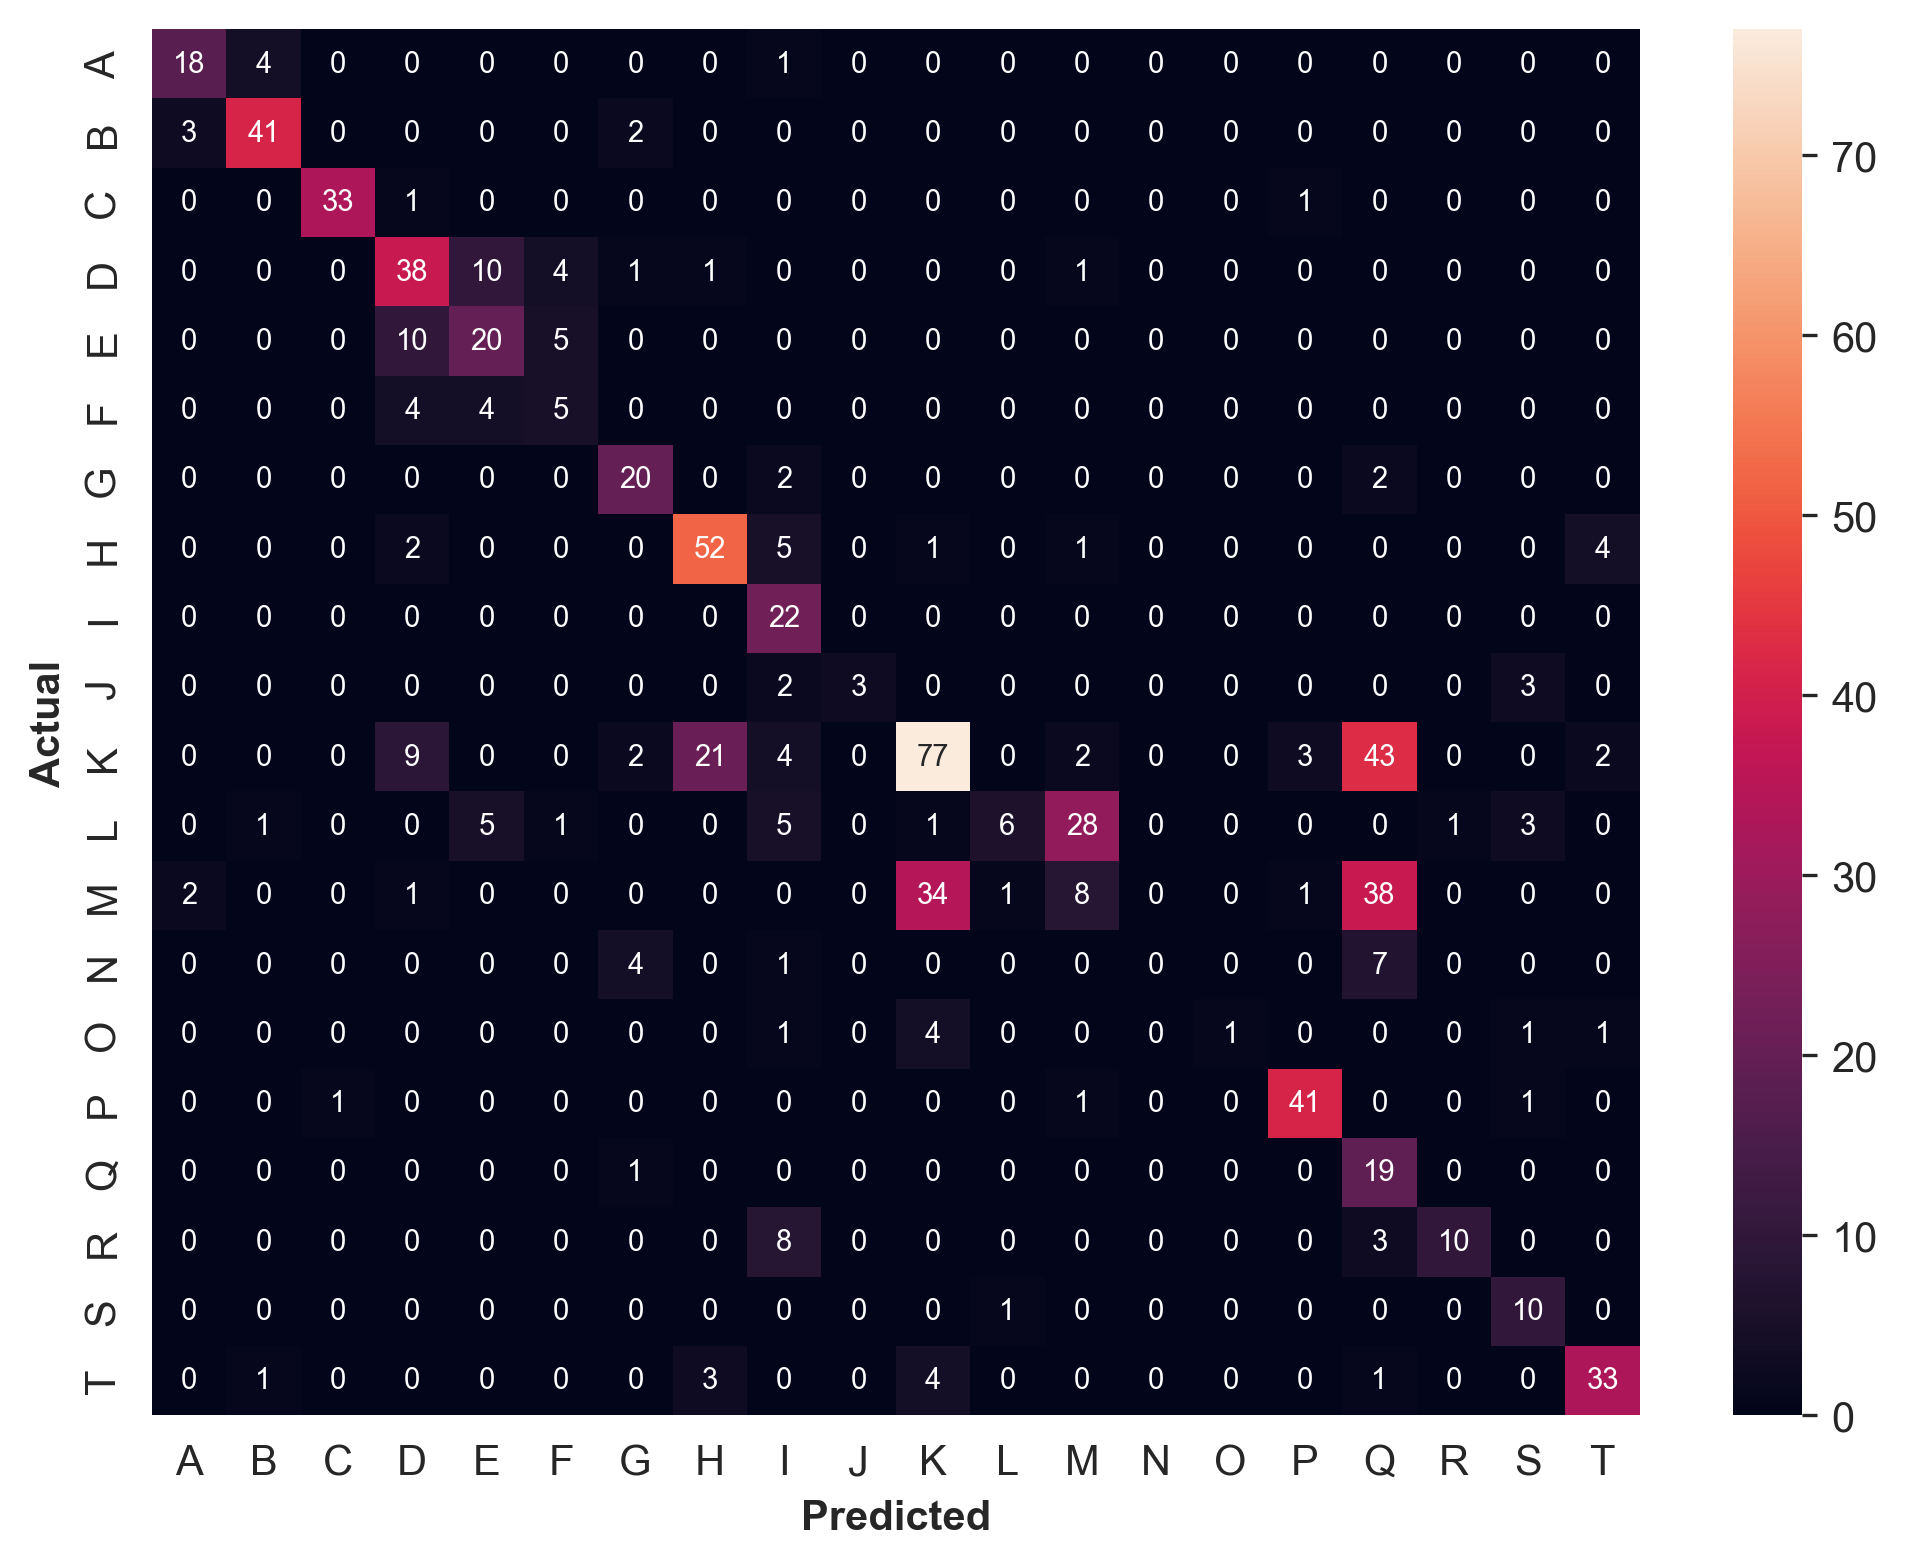
\includegraphics[width=\textwidth]
        {figures/experiment1-conf-matrix-resnet50.png}
        \caption{\texttt{resnet50}}
    \end{subfigure}%
    \begin{subfigure}{.33\textwidth}
        \centering
        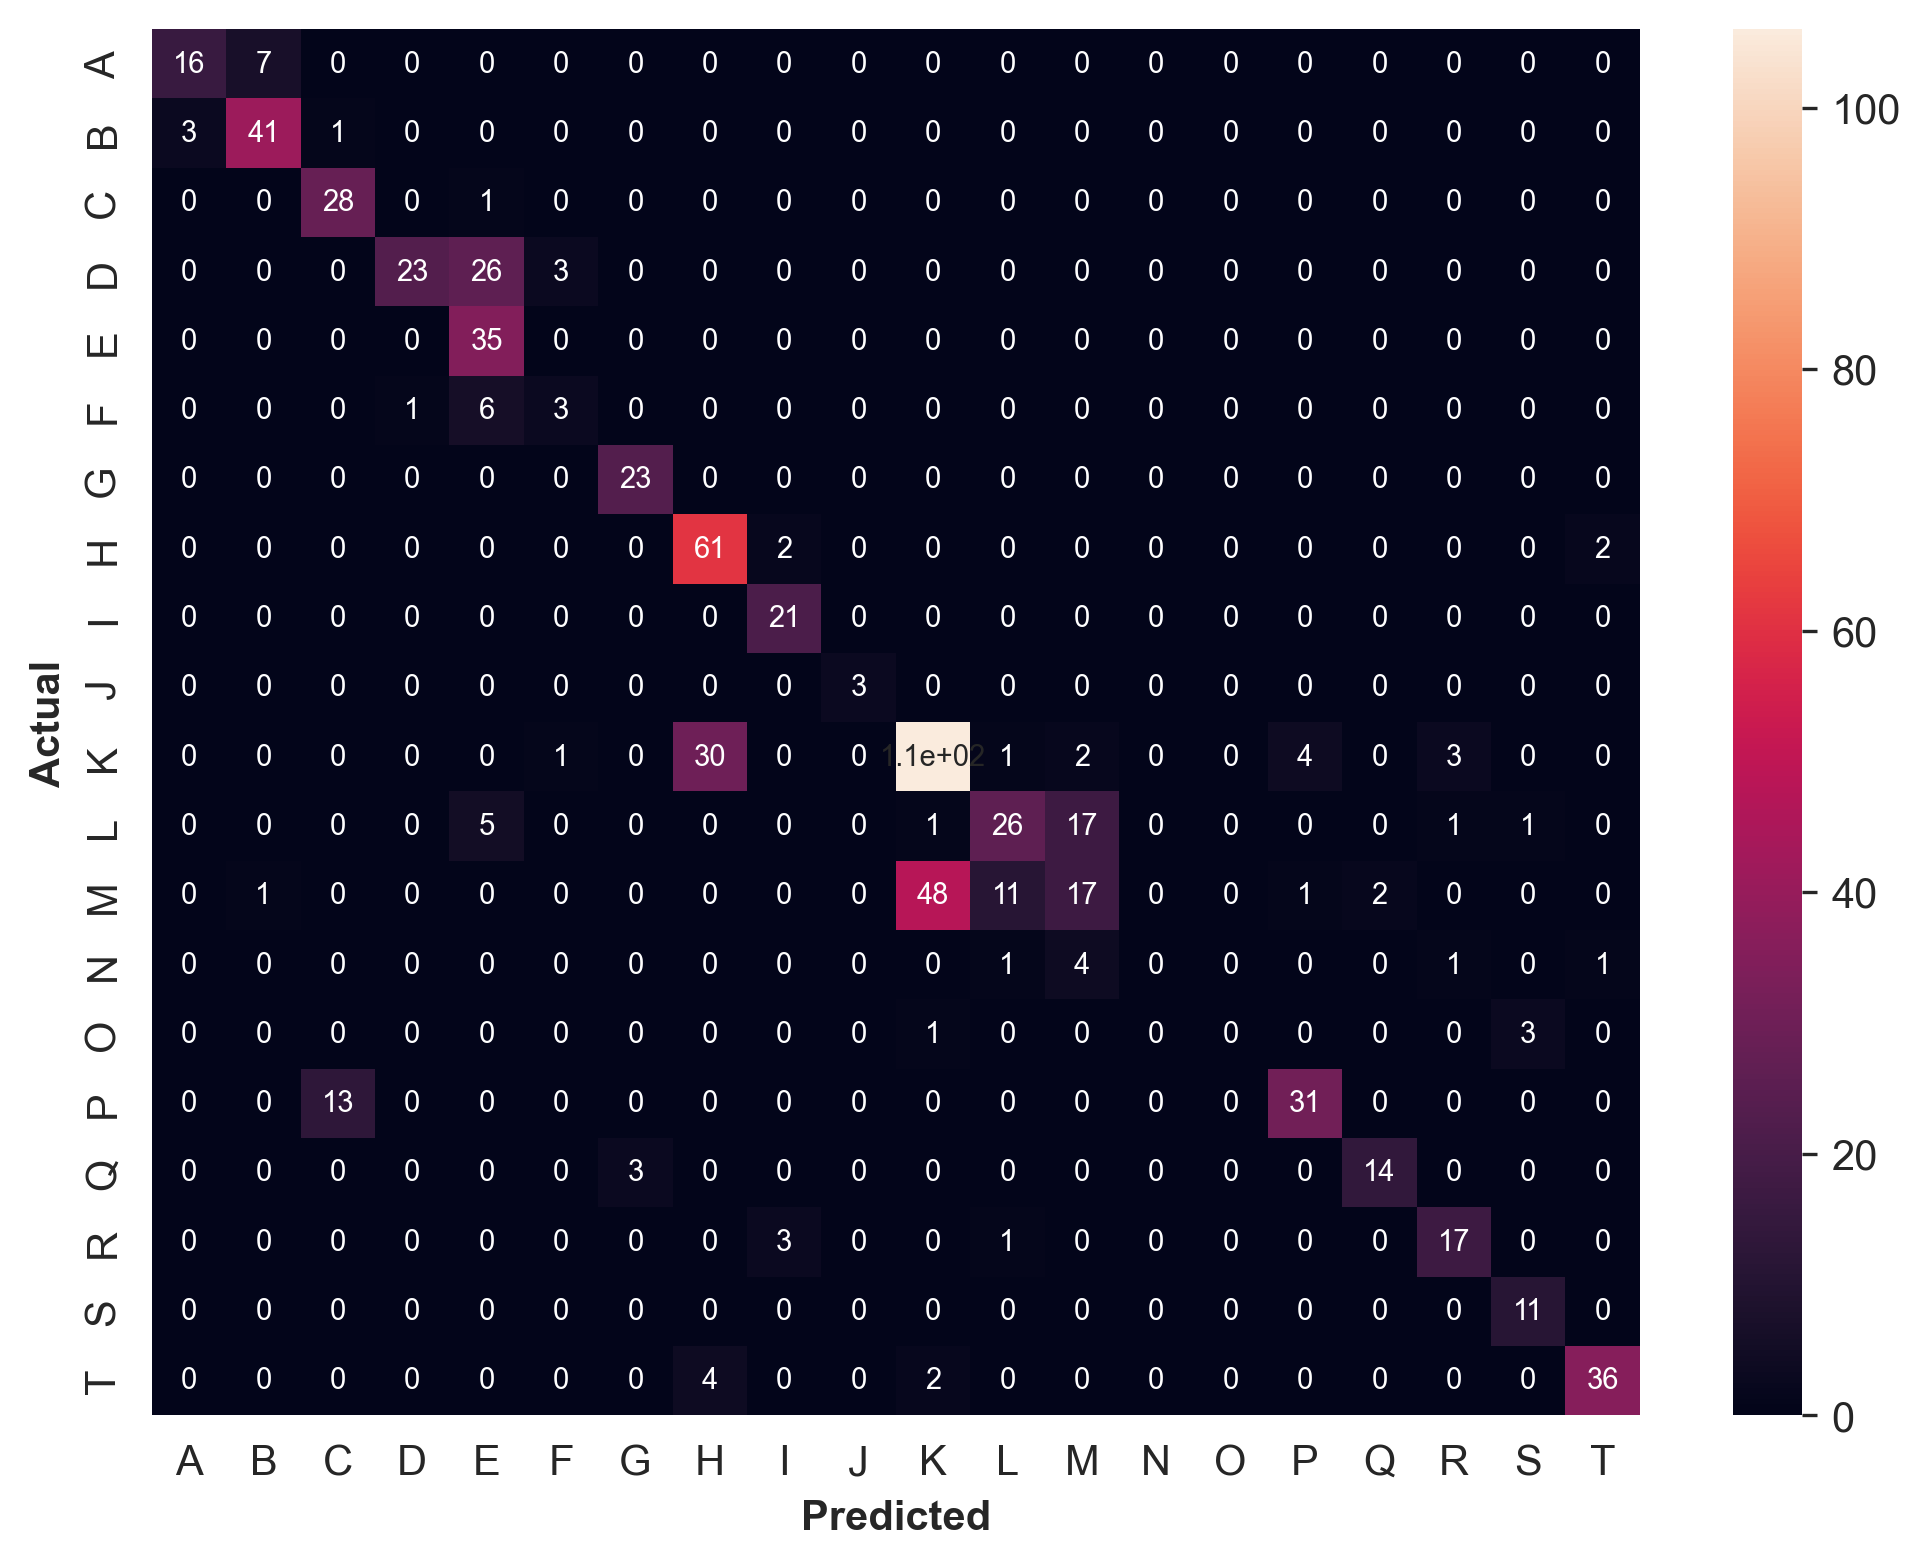
\includegraphics[width=\textwidth]
        {figures/experiment1-conf-matrix-resnet18-rnn.png}
        \caption{\texttt{resnet18-rnn}}
    \end{subfigure}
    \begin{subfigure}{.33\textwidth}
        \centering
        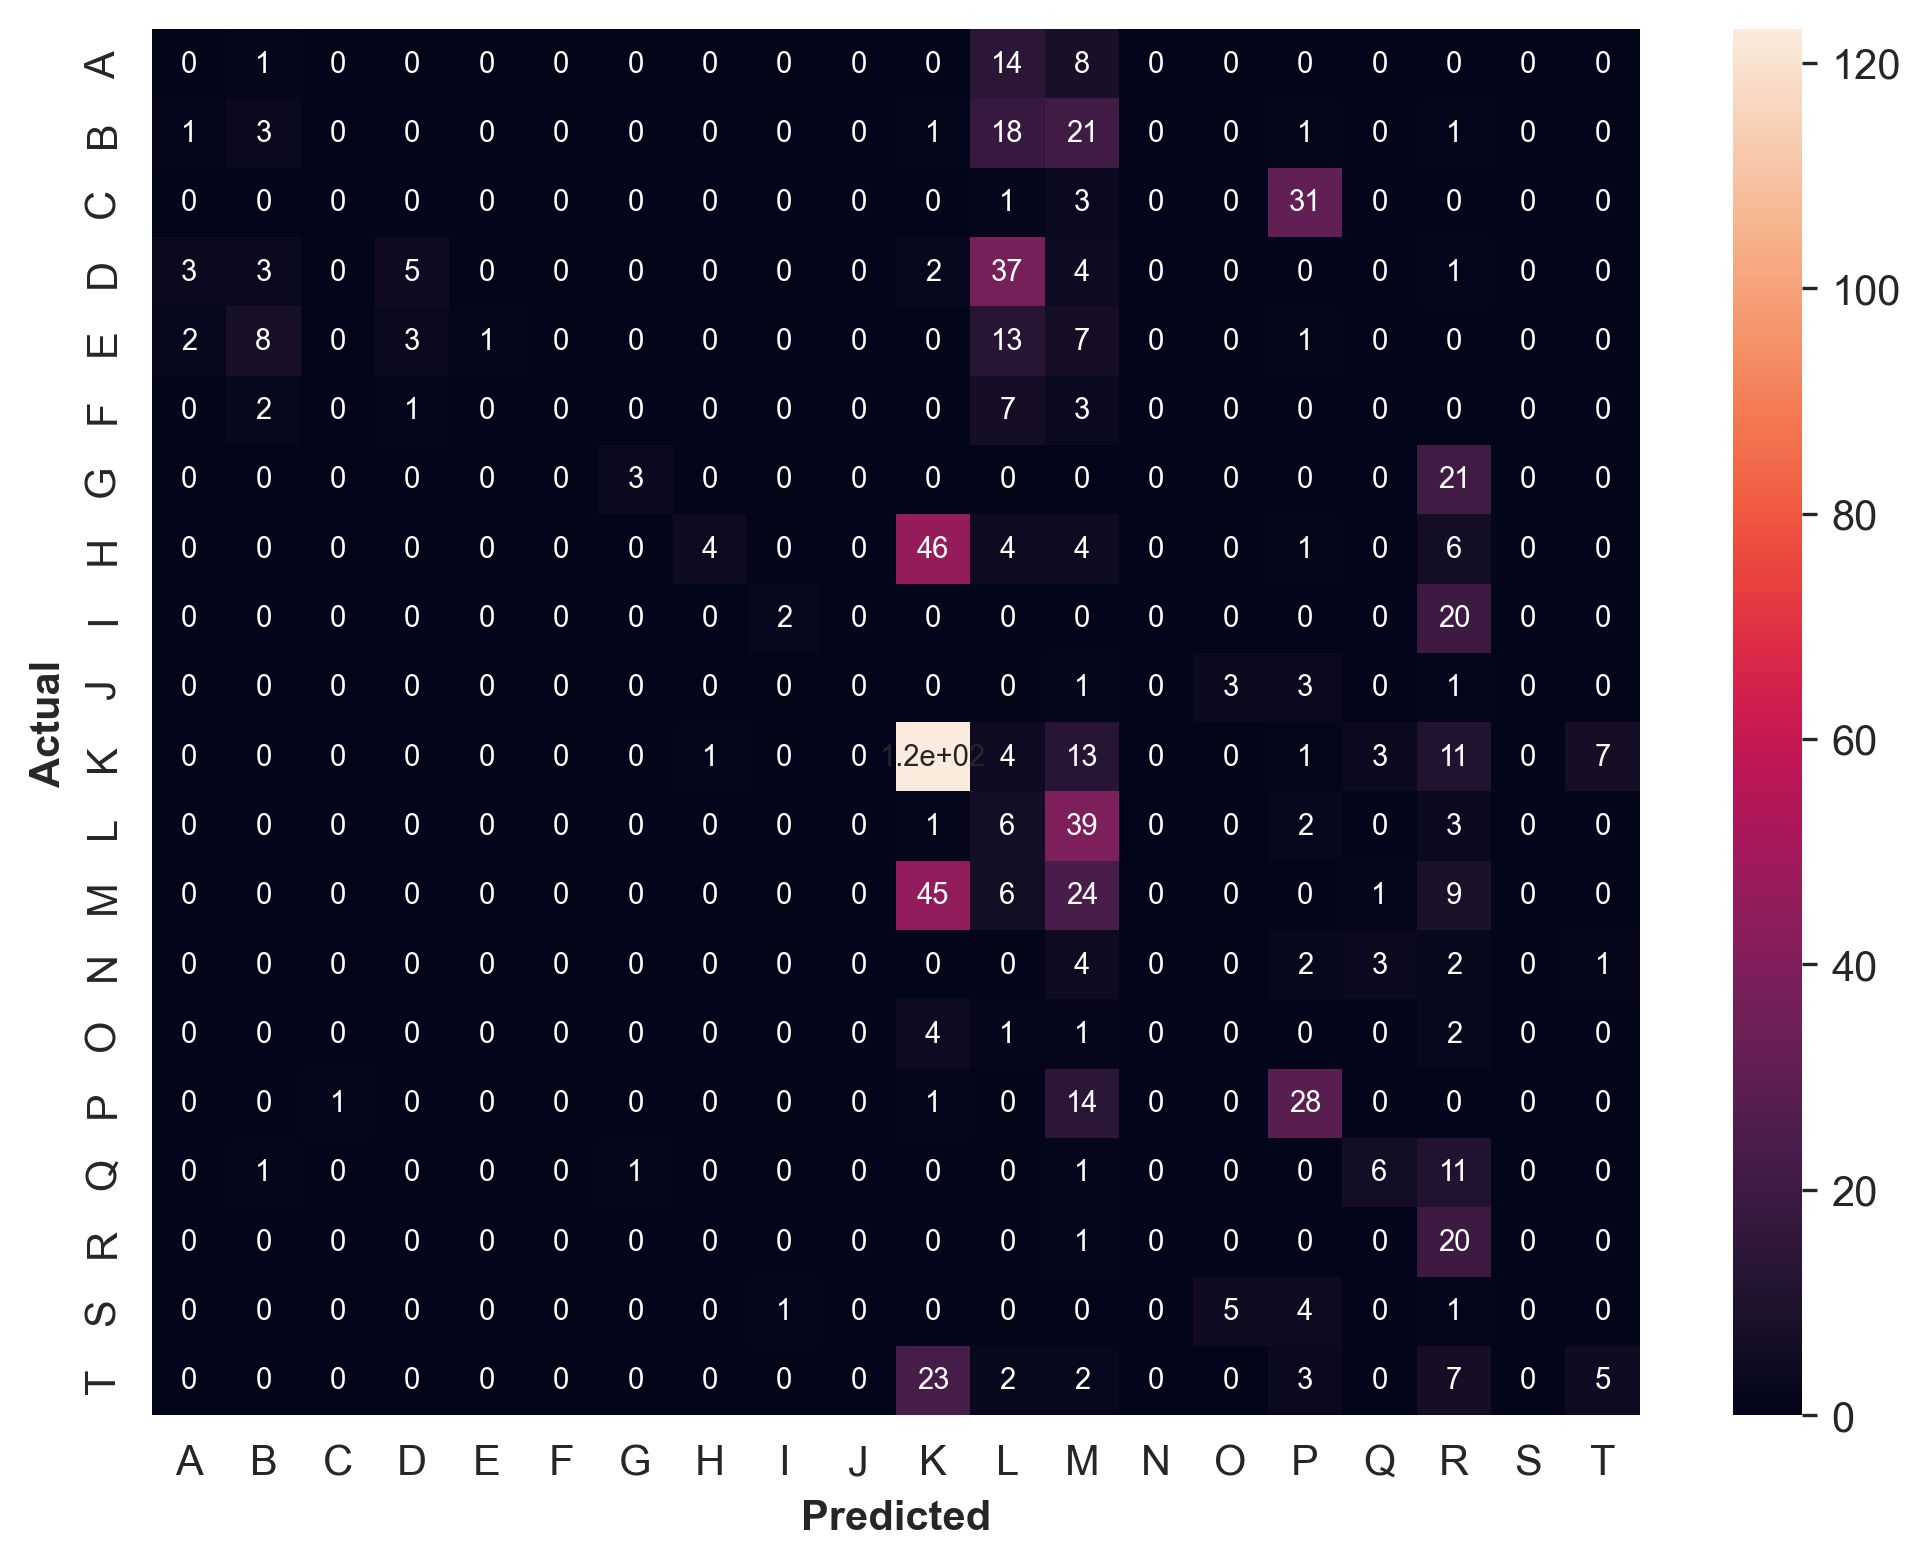
\includegraphics[width=\textwidth]
        {figures/experiment1-conf-matrix-mobilenet_v3_small.png}
        \caption{\texttt{mobilenet\_v3\_small}}
    \end{subfigure}%
    \begin{subfigure}{.33\textwidth}
        \centering
        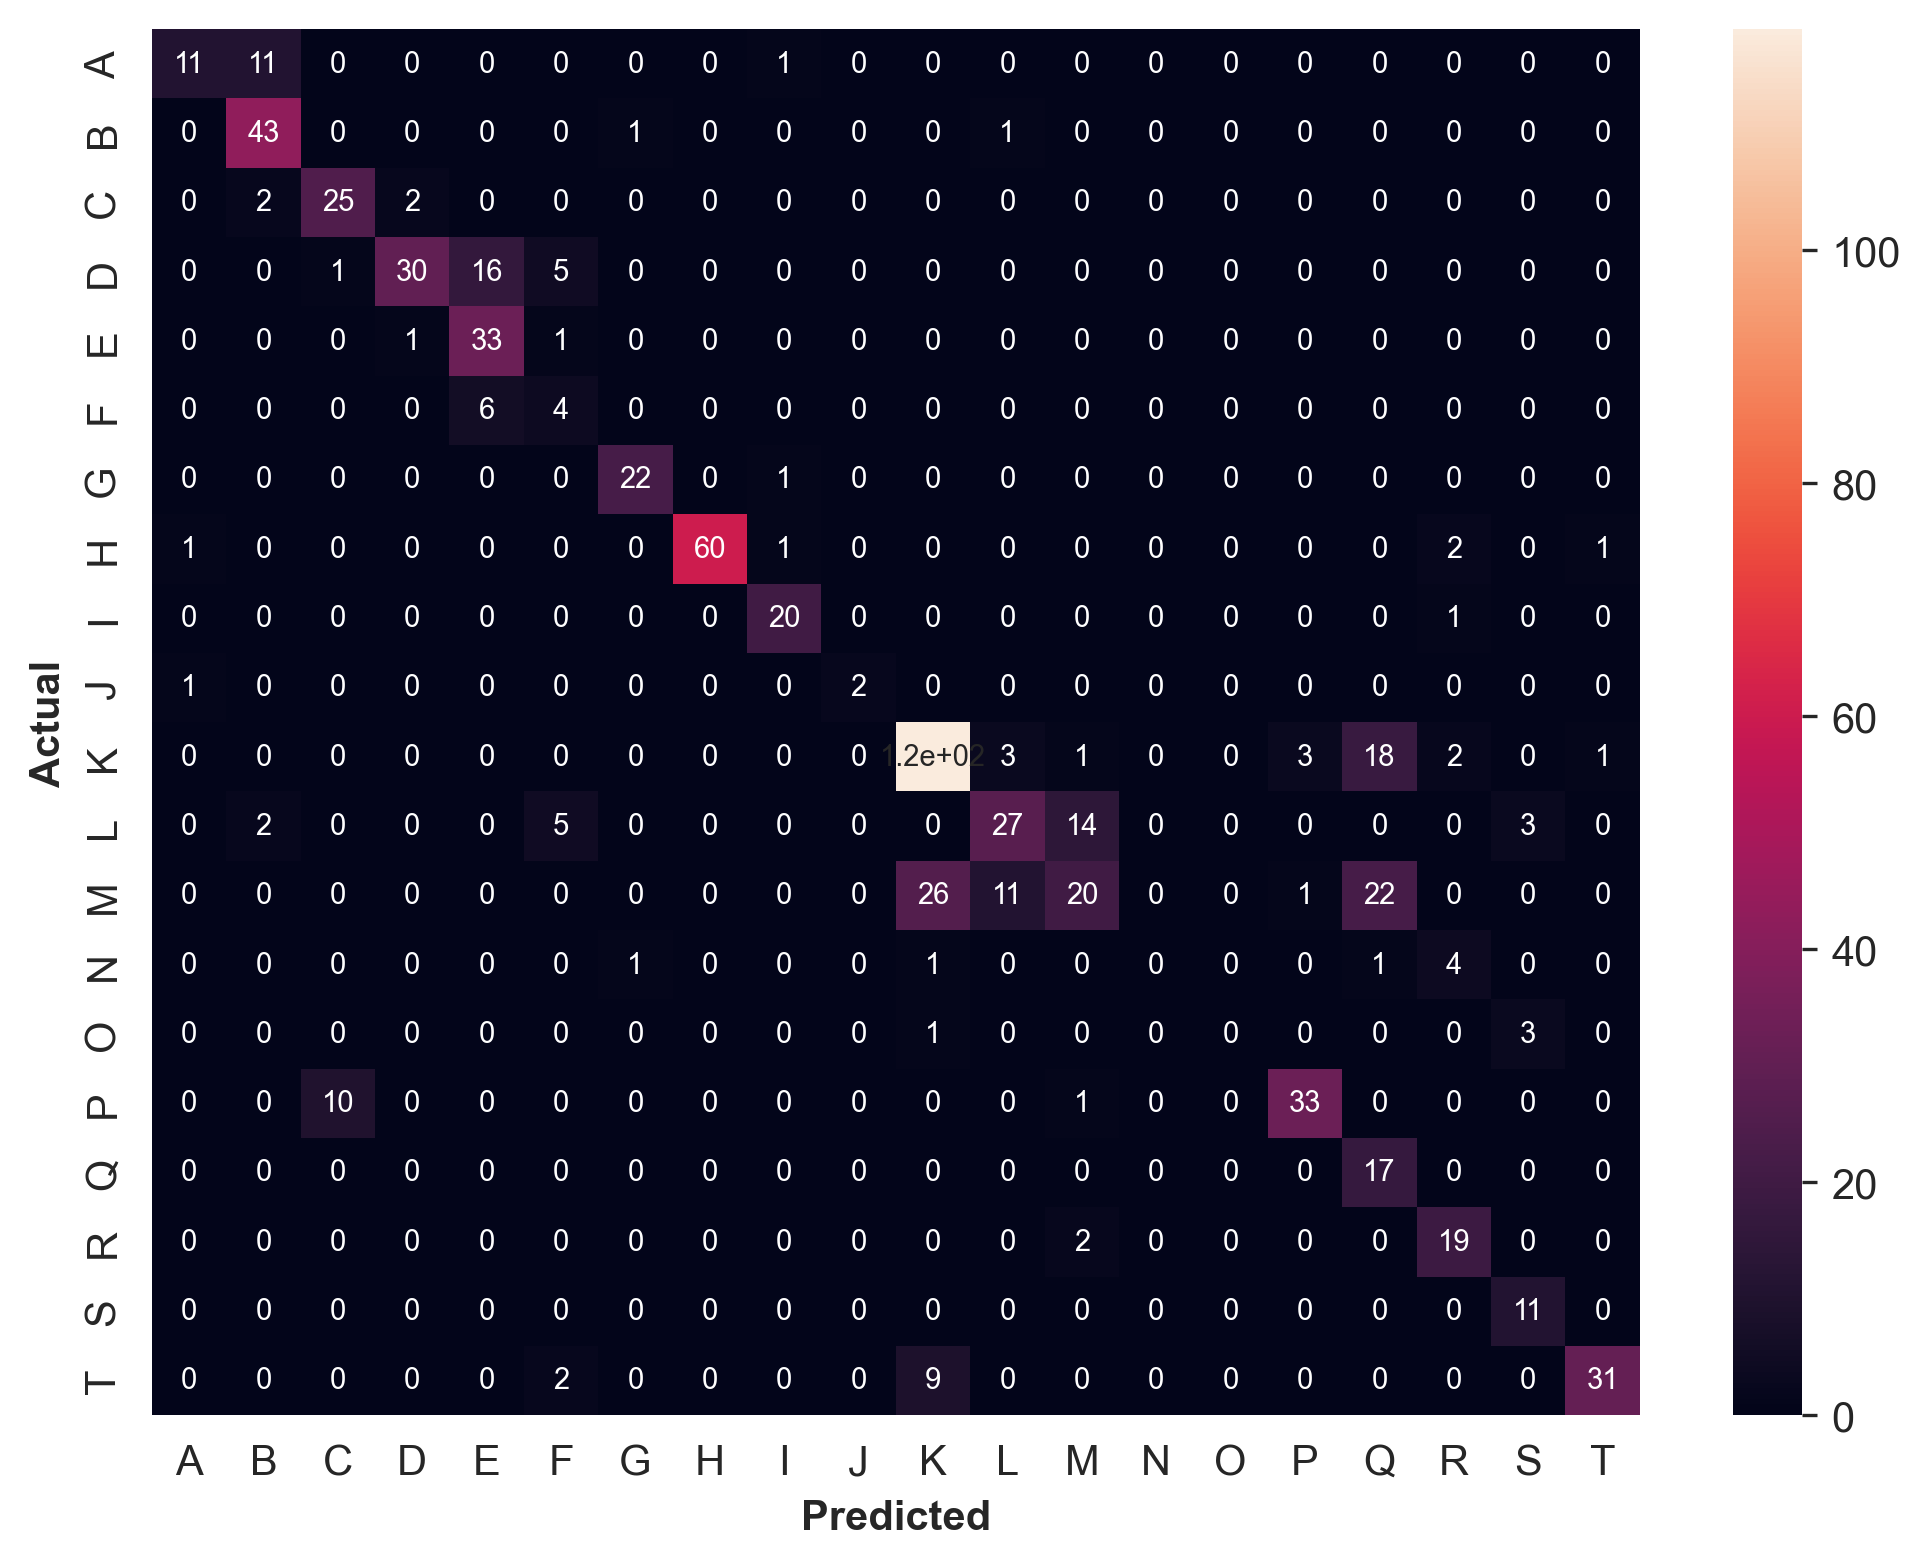
\includegraphics[width=\textwidth]
        {figures/experiment1-conf-matrix-resnet18-lstm.png}
        \caption{\texttt{resnet18-lstm}}
    \end{subfigure}%

    \caption{
      \textbf{Confusion Matrices.} The table shows the (unnormalised) confusion
      matrices of all models in Experiment 1. The predictions are computed on
      the frames from the test split and the matrix. The entry at index $(i,j)$
      is the number of samples with true class $i$ that were predicted to be
      class $j$.
    }

    \label{fig:conf-matrices-experiment1}
  \end{figure}

  \newpage
  \restoregeometry

  % section appendix (end)
  

\end{document}
